% Documents setup
\documentclass[11pt]{book}

% fix for pandoc 1.14
\providecommand{\tightlist}{%
  \setlength{\itemsep}{0pt}\setlength{\parskip}{0pt}}

\usepackage{tabu} % https://tex.stackexchange.com/questions/50332/vertical-spacing-of-a-table-cell

% Location of the csas-style repository: adjust path as needed
\newcommand{\locRepo}{csas-style}

% Use the style file in the csas-style repository (res-doc.sty)
\usepackage{\locRepo/res-doc}

% header-includes from R markdown entry


% Headers and footers
\lhead{}
% \lhead{}
\rhead{}
% \rfoot{DRAFT - DO NOT CITE}

%%%% Commands for title page etc %%%%%

% Publication year
\newcommand{\rdYear}{2024}

% Publication month
\newcommand{\rdMonth}{Month}

% Report number
\newcommand{\rdNumber}{2024/063}

% Region
\newcommand{\rdRegion}{Pacific Region}

% Title
\newcommand{\rdTitle}{Estimating Precautionary Approach Reference Points and Assessing Consequences of Harvest Control Rules for Fraser River Pink Salmon (\emph{Oncorhynchus gorbuscha})}

\newcommand{\rdISBN}{978-0-660-38322-4}
\newcommand{\rdCatNo}{Fs70-6/2021-012E-PDF}

% Author names separated by commas and ', and' for the last author in the format 'M.H. Grinnell' (use \textsuperscript{n} for addresses)
\newcommand{\rdAuth}{Dylan M. Glaser\textsuperscript{1} Brendan M. Connors\textsuperscript{2} Kaitlyn Dionne\textsuperscript{3} and Ann-Marie Huang\textsuperscript{4}}

% Author names reversed separated by commas in the format 'Grinnell, M.H.'
\newcommand{\rdAuthRev}{Glaser, D.M., Connors, B.M., Dionne, K., and Huang, A.M.}

% Author addresses (use \textsuperscript{n})
\newcommand{\rdAuthAddy}{\textsuperscript{1}Pacific Biological Station\\
Fisheries and Oceans Canada, 3190 Hammond Bay Road\\
Nanaimo, British Columbia, V9T 6N7, Canada\\
\smallskip \textsuperscript{2}Institute of Ocean Sciences\\
Fisheries and Oceans Canada, 9860 W Saanich Road\\
Sidney, British Columbia, V8L 5T5, Canada\\
\smallskip \textsuperscript{3}Kamloops Office\\
Fisheries and Oceans Canada, 985 McGill Pl\\
Kamloops, British Columbia, V2C 6X6, Canada\\
\smallskip \textsuperscript{4}Regional Headquarters (Pacific)\\
Fisheries and Oceans Canada, 200-401 Burrard Street\\
Vancouver, British Columbia, V6C 3S4, Canada\\}

\newcommand{\citationOtherLanguage}{Glaser, D.M., Connors, B.M., Dionne, K., et Huang, A.M. Estimation de précaution Points de référence d'approche et évaluation des conséquences des règles de contrôle des prises pour Saumon rose du fleuve Fraser (\emph{Oncorhynchus gorbuscha}). DFO Secr. can. des avis sci. du MPO. Doc. de rech 2024/nnn. iv + 13 p.}

% Name of file with abstract and resume (see \abstract in inst/csas-style/res-doc.sty)
\newcommand{\rdAbstract}{\abstract{Fraser River Pink Salmon spawn throughout the Fraser Basin in odd-numbered years and the Stock Management Unit is comprised of a single Conservation Unit. Landslides have occurred causing migratory impediments to returning adults at different periods with the most notable being Hells Gate in 1914 and more recently the Big Bar Landslide discovered in 2019. Fraser Pink Salmon marine survival is associated with sea-surface temperatures during early marine life, spring bloom timing, and the North Pacific Current, all of which are expected to change as the North Pacific warms as a result of climate change. Adult body size has declined over time, coincident with increasing abundances of salmon in the North Pacific, which has the potential to impact reproductive output as fecundity scales with female size. We fit a state-space spawner-recruitment model to available data to characterize stock dynamics and derive estimates of biological reference points to assess stock status. We then developed a simple closed-loop simulation model based on recent estimates of productivity to quantify future expected biological and fishery performance of the current harvest control rule (HCR), an illustrative alternative HCR and a no fishing scenario. We estimated the proposed Upper Stock Reference (USR) point of 80\% \(S_{MSY}\) to be 4.6 million (M) fish (3.64-6.11M; median and 80th percentiles), the Limit Reference Point (LRP) \(S_{gen}\) to be 1.72M (1.10-2.70M), and the maximum removal reference rate (RR), \(U_{MSY}\) to be 0.56 (0.47-0.63). The most recent (2023) observed estimate of spawner abundance for Fraser Pink Salmon is 9.58M and we conclude that the Stock Management Unit is in a ``healthy'' state. The existing HCR for Fraser Pinks has a very low probability (\textless{} 5\%) of the stock falling below its LRP, and a relatively high probability (87.5\%) of spawner abundance being above the USR over the next 10 years. Assuming fisheries fully utilize allowable catch, median annual catch is projected to be 10.3M over the same time period. Assessment of an illustrative alternative HCR, which is strictly compliant with DFO's Precautionary Approach Framework, had similar biological performance and slightly worse fishery performance. The results of a robustness test, where productivity was reduced to 10\% of its recent estimate, showed that the current and alternate HCRs had a 9\% and 20\% chance, respectively, of the stock falling below its LRPs over the next 10 years. We conclude with recommendations on re-assessment triggers and potential areas to focus future work.}}

%%%% End of title page commands %%%%%

% \pdfcompresslevel=5 % faster PNGs

\setcounter{section}{0}

\bibliographystyle{csas-style/res-doc}

\usepackage{amsmath}
\usepackage{bm}

% commands and environments needed by pandoc snippets
% extracted from the output of `pandoc -s`
%% Make R markdown code chunks work
\usepackage{array}
\usepackage{amssymb,amsmath}
\usepackage{color}
\usepackage{fancyvrb}

% From default template:
\newcommand{\VerbBar}{|}
\newcommand{\VERB}{\Verb[commandchars=\\\{\}]}
\DefineVerbatimEnvironment{Highlighting}{Verbatim}{commandchars=\\\{\},formatcom=\color[rgb]{0.00,0.00,0.00}}
\usepackage{framed}
\definecolor{shadecolor}{RGB}{248,248,248}
\newenvironment{Shaded}{\begin{snugshade}}{\end{snugshade}}
\newcommand{\AlertTok}[1]{\textcolor[rgb]{0.94,0.16,0.16}{#1}}
\newcommand{\AnnotationTok}[1]{\textcolor[rgb]{0.56,0.35,0.01}{\textbf{\textit{#1}}}}
\newcommand{\AttributeTok}[1]{\textcolor[rgb]{0.77,0.63,0.00}{#1}}
\newcommand{\BaseNTok}[1]{\textcolor[rgb]{0.00,0.00,0.81}{#1}}
\newcommand{\BuiltInTok}[1]{#1}
\newcommand{\CharTok}[1]{\textcolor[rgb]{0.31,0.60,0.02}{#1}}
\newcommand{\CommentTok}[1]{\textcolor[rgb]{0.56,0.35,0.01}{\textbf{#1}}}
\newcommand{\CommentVarTok}[1]{\textcolor[rgb]{0.56,0.35,0.01}{\textbf{\textit{#1}}}}
\newcommand{\ConstantTok}[1]{\textcolor[rgb]{0.00,0.00,0.00}{#1}}
\newcommand{\ControlFlowTok}[1]{\textcolor[rgb]{0.13,0.29,0.53}{\textit{#1}}}
\newcommand{\DataTypeTok}[1]{\textcolor[rgb]{0.13,0.29,0.53}{#1}}
\newcommand{\DecValTok}[1]{\textcolor[rgb]{0.00,0.00,0.81}{#1}}
\newcommand{\DocumentationTok}[1]{\textcolor[rgb]{0.56,0.35,0.01}{\textbf{\textit{#1}}}}
\newcommand{\ErrorTok}[1]{\textcolor[rgb]{0.64,0.00,0.00}{\textit{#1}}}
\newcommand{\ExtensionTok}[1]{#1}
\newcommand{\FloatTok}[1]{\textcolor[rgb]{0.00,0.00,0.81}{#1}}
\newcommand{\FunctionTok}[1]{\textcolor[rgb]{0.00,0.00,0.00}{#1}}
\newcommand{\ImportTok}[1]{#1}
\newcommand{\InformationTok}[1]{\textcolor[rgb]{0.56,0.35,0.01}{\textbf{\textit{#1}}}}
\newcommand{\KeywordTok}[1]{\textcolor[rgb]{0.13,0.29,0.53}{\textit{#1}}}
\newcommand{\NormalTok}[1]{#1}
\newcommand{\OperatorTok}[1]{\textcolor[rgb]{0.81,0.36,0.00}{\textit{#1}}}
\newcommand{\OtherTok}[1]{\textcolor[rgb]{0.56,0.35,0.01}{#1}}
\newcommand{\PreprocessorTok}[1]{\textcolor[rgb]{0.56,0.35,0.01}{\textbf{#1}}}
\newcommand{\RegionMarkerTok}[1]{#1}
\newcommand{\SpecialCharTok}[1]{\textcolor[rgb]{0.00,0.00,0.00}{#1}}
\newcommand{\SpecialStringTok}[1]{\textcolor[rgb]{0.31,0.60,0.02}{#1}}
\newcommand{\StringTok}[1]{\textcolor[rgb]{0.31,0.60,0.02}{#1}}
\newcommand{\VariableTok}[1]{\textcolor[rgb]{0.00,0.00,0.00}{#1}}
\newcommand{\VerbatimStringTok}[1]{\textcolor[rgb]{0.31,0.60,0.02}{#1}}
\newcommand{\WarningTok}[1]{\textcolor[rgb]{0.56,0.35,0.01}{\textbf{\textit{#1}}}}

\newcommand{\lt}{\ensuremath <}
\newcommand{\gt}{\ensuremath >}

%Defines cslreferences environment
%Required by pandoc 2.8
%Copied from https://github.com/rstudio/rmarkdown/issues/1649
% % \newlength{\cslhangindent}
% \setlength{\cslhangindent}{1.5em}
% \newenvironment{cslreferences}%
%   {}%
%   {\par}
% 
\DeclareGraphicsExtensions{.png,.pdf}
\begin{document}

\frontmatter

\hypertarget{introduction}{%
\section{INTRODUCTION}\label{introduction}}

\hypertarget{background}{%
\subsection{BACKGROUND}\label{background}}

\hypertarget{fraser-river-pink-salmon}{%
\subsubsection{Fraser River Pink Salmon}\label{fraser-river-pink-salmon}}

The Fraser River is a large free-flowing river that is 1375 kilometers long and drains 233,000 square kilometers. The basin has a wide diversity of habitats that have been divided into several distinct regions including two on the mainstem of the Fraser, one in Lillooet, and three in the Thompson drainage (\protect\hyperlink{ref-holtbyConservationUnitsPacific2008}{{``Conservation {Units} for {Pacific Salmon} under the {W}ild {S}almon {P}olicy''} In press}). The Fraser River is home to all five species of Pacific salmon and most of their life history variants. The environmental complexity of the Fraser River, and the diversity of the salmon populations within it, has underpinned indigenous food security for millennia (\protect\hyperlink{ref-nesbittSpeciesPopulationDiversity2016}{Nesbitt and Moore 2016}) and likely contributed to the resilience of salmon populations to environmental disturbances through time.

Fraser River Pink Salmon (\emph{Oncorhynchus gorbuscha}) spawn on odd years in the Fraser River at great abundances. Currently, the largest aggregate of Pink Salmon spawns in the lower Fraser watershed. However, prior to the slide at Hells Gate, Fraser River Pink Salmon spawned at greater abundances in the upper Fraser watershed with significant populations in the Thompson and Seton systems (\protect\hyperlink{ref-pessInfluencePopulationDynamics2012}{Pess et al. 2012}). Pink Salmon fry migrate to the ocean in the spring, adults spend approximately 18 months at sea, then return to the Fraser River from mid-August to early October to spawn (\protect\hyperlink{ref-dfoSouthernSalmonIntegrated2023}{DFO 2023}). This obligate 2 year life cycle exhibited by Pink Salmon results in even and odd year cohorts that are reproductively isolated from each other and density-dependent interactions between odd and even lineages likely often contributes to one cycle line being numerically dominant over the other (\protect\hyperlink{ref-krkosek2011cycles}{Krkošek et al. 2011}). The even year Pink return to the Fraser is negligible, not assessed, and not part of this CU.

Fraser River Pink Salmon migrate to the Fraser River estuary shortly after emergence and spend several months feeding in the Strait of Georgia before migrating as far north as the Gulf of Alaska where they reside for approximately one year (\protect\hyperlink{ref-dfoFraserRiverSalmon1998}{DFO 1998}). When Fraser Pinks return to the Fraser River from the North Pacific, a portion of the run migrates around the northern tip of Vancouver Island through Johnstone Strait, while others move around the southern tip through the Strait of Juan de Fuca; this ratio of northern to southern migration is known as the diversion rate (\protect\hyperlink{ref-folkesEvaluatingModelsForecast2018}{Folkes et al. 2018}). This diversion rate is increasingly dominated by Pink Salmon taking the northern migration route, which affects the accuracy of run size estimates as a result of differential encounters with test fisheries (\protect\hyperlink{ref-hagueMovingTargetsAssessing2021}{Hague et al. 2021}). Changes in diversion rate could also have implications for survival via encounters with prey, predators, pathogens, and co-occurring species as a result of differing densities of fish farms on either side of Vancouver Island (\protect\hyperlink{ref-grantSummaryFraserRiver2018}{Grant et al. 2018}).

\hypertarget{spawners-and-catch}{%
\subsubsection{Spawners and Catch}\label{spawners-and-catch}}

Data on catch and spawner abundance (i.e., escapement) has been collected for well over a century, with indices of abundance recorded back to 1901 (\protect\hyperlink{ref-rickerHistoryPresentState1989}{Ricker 1989}). However, consistent and reliable spawner and catch data are only available from 1959 to present. More details on catch and spawner data used in this report are provided in the Data Sources section.

\hypertarget{enhancement}{%
\subsubsection{Enhancement}\label{enhancement}}

Enhancement of Fraser Pinks is limited and has primarily occurred via spawning channels to create additional high quality spawning habitat. Records dating back to brood year 1955 show estimates of several million Pink fry migrating out of spawning channels (see data in the repository linked in Supplement A). Estimates of outmigration varied in precision with monitoring programs primarily designed for other species. Rotary screw trap sampling and or egg to fry survival estimates were used to generate release numbers. Prior to the establishment of the Salmonid Enhancement Program (SEP), salmonid enhancement facilities on the Fraser were managed by the International Pacific Salmon Fishing Commission (IPSFC) and production was limited to incidental stocking in spawning channels (i.e.~Seaton, Jones, and Weaver). Following the establishment of SEP in 1977 Fraser Pink began to be enhanced in hatcheries where fish would be incubated and reared in a facility to maximize incubation, egg, and fry survivals. Due to their limited time spent in freshwater, Pinks require less resources to enhance relative to other Pacific salmon; a characteristic that has made them a popular fish to raise for marine catch. SEP is currently re-evaluating stocking practices, and has reduced the number of fed fry produced since the late 2000's (Figure~\ref{fig:fig-hatch-cont}), partly due to reduced catch opportunities, and evolving priorities.

\hypertarget{current-management-and-trends}{%
\subsubsection{Current Management and Trends}\label{current-management-and-trends}}

The current harvest control rule (HCR) for Fraser Pink Salmon was first implemented in 1987. It consists of three management zones: 1) at run sizes below 7.059 million (M) Pinks, the the maximum allowable exploitation rate increases from 0\% when there are no Pink Salmon to 15\% at 7.059M Pinks, 2) at run sizes between 7.059 and 20M Pinks, there is a fixed spawner abundance goal of 6M, and 3) at run sizes greater than 20M Pinks, the maximum exploitation rate is 70\%. Documentation of the rationale for the current HCR has been difficult to locate, but a handwritten International Pacific Salmon Fisheries Commission memo from 1983 appears to calculate an egg deposition target of 5 billion eggs that would generate desired production and associated adult spawner target, assuming an average weight, that would meet the egg deposition target (S. Latham, Pacific Salmon Commission {[}PSC{]}, Vancouver, British Columbia, pers. comm.), Ricker (\protect\hyperlink{ref-rickerHistoryPresentState1989}{1989}) also estimates \(U_{MSY}\) at 70\% which may have supported the current target Removal Reference rate (RR)(Figure~\ref{fig:fig-HCRs}).

Additional management measures are often taken during fisheries directed on Fraser Pink Salmon to avoid stocks of concern where possible and to reduce impacts on co-migrating stocks of concern when it is not. Measures taken to reduce Sockeye bycatch have included: time and area closures (e.g., Interior Fraser Coho fishing window closure), gear requirements (e.g., use of beach seines or shallow seines instead of drift gill nets, bait ban for recreational fisheries), and operational changes (e.g., brailing requirements and maximum recommended set sizes for purse seines).

In the 14 returns of Fraser Pinks prior to implementation of the 1987 HCR (i.e., spanning 1959-1985), the average run size was 9.3M, average spawner abundance was 2.5M, and the average exploitation rate was 69\%. In the 19 years of Fraser Pinks returns since the implementation of the HCR (1987-2023), there have been two years when the HCR exploitation rate limit was exceeded (1987 and 1997), the average run size was 12.9M, the average spawner abundance was 9.4M, and the average exploitation rate was 25\%. Overall, Fraser Pink returns may be characterized as ``variable, but stable''. In the last five generations (10 years, 5 returns), the run size and spawner abundance have been slightly increasing with low interannual variability, with an average run size of 7.38M, average spawner abundances of 6.89M, and an average exploitation rate of 6\% (Figure~\ref{fig:fig-catch-esc}).

\hypertarget{fraser-pink-fisheries-and-fish-stocks-provisions}{%
\subsubsection{Fraser Pink Fisheries and Fish Stocks Provisions}\label{fraser-pink-fisheries-and-fish-stocks-provisions}}

Canada's \emph{Fisheries Act} was amended in June 2019. It included new requirements under the Fish Stocks Provisions (FSP), which states that ``\emph{the Minister shall implement measures to maintain major fish stocks at or above the level necessary to promote the sustainability of the stock, taking into account the biology of the fish and the environmental conditions affecting the stock}'' (\protect\hyperlink{ref-DFO1985Act}{DFO 1985}). Fraser Pink Salmon has been identified as a major fish stock and to assist with the implementation of the FSP, the authors working in conjunction with DFO Fisheries Management have identified candidate values for the aggregate-based component of the Limit Reference Point (LRP), the Upper Stock Reference point (USR) and the maximum Removal Reference point (RR). Increasing concern about potential impacts from climate change (e.g.~warming ocean temperature, freshwater flooding events; MacDonald and Grant (\protect\hyperlink{ref-macdonaldStateCanadianPacific2023}{2023})), potential for increasing inter- and intra-specific competition in the ocean (\protect\hyperlink{ref-ruggeroneNumbersBiomassNatural2018}{Ruggerone and Irvine 2018}; \protect\hyperlink{ref-ruggeroneDiatomsKillerWhales2023}{Ruggerone et al. 2023}), and evidence of changing demographics (\protect\hyperlink{ref-pacificsalmoncommissionPSCBiologicalData2023}{Pacific Salmon Commission 2023}) all underscore the need to update our understanding of stock dynamics and status. The relationship between Fraser Pink population dynamics and management haven't been assessed in over 30 years (last DFO assessment Ricker (\protect\hyperlink{ref-rickerHistoryPresentState1989}{1989})), partly due to concerns about calibration among spawner assessment methodologies (\protect\hyperlink{ref-grantFraserRiverPink2014}{Grant et al. 2014}). The new FSP requirements necessitate a careful re-examination of population dynamics and the sustainability of the current HCR.

\hypertarget{objectives}{%
\subsection{OBJECTIVES}\label{objectives}}

As the Fraser Pink Salmon Stock Management Unit (SMU) is comprised of a single Conservation Unit, we use DFO's Wild Salmon Policy benchmarks, which should be biologically based and explicitly account for uncertainty (\protect\hyperlink{ref-dfoCanadaPolicyConservation2005}{DFO 2005}, \protect\hyperlink{ref-dfoFisheryDecisionmakingFramework2009}{2009}), to identify candidate FSP reference points.

The objectives are to:
\begin{enumerate}
\def\labelenumi{\arabic{enumi}.}
\item
  describe current understanding of: (a) stock structure and distribution, (b) stock status and trends, and (c) ecosystem and climate factors affecting the stock;
\item
  provide estimates of: (a) candidate reference points and (b) the expected biological and fishery performance of current and alternative harvest control rules;
\item
  propose exceptional circumstances or assessment triggers for the stock; and
\item
  identify areas requiring future work.
\end{enumerate}
\hypertarget{stock-structure-and-distribution}{%
\section{STOCK STRUCTURE AND DISTRIBUTION}\label{stock-structure-and-distribution}}

Fraser River Pink Salmon predominantly spawn in the lower portion of the Fraser Basin, below the Fraser Canyon and Hells Gate (Figure~\ref{fig:fig-map}). However, there is a large component of the stock that returns to the Thompson River and the Seton-Anderson complex. Before the slide at Hells Gate in 1914, most of the Fraser River Pink Salmon run returned and spawned in the upper Fraser River (\protect\hyperlink{ref-pessInfluencePopulationDynamics2012}{Pess et al. 2012}). Although there is a lack of abundance data at the tributary level in recent decades for Fraser Pink Salmon, assessment observations from other species have persistently noted Pink Salmon in the Quesnel, Chilcotin, and the Nechako Rivers. In 2019, DFO was alerted to a landslide in the middle Fraser near Big Bar. Pink Salmon were noted as being among the species delayed in their upstream migration by the slide. Slide mitigation efforts have largely been successful and Pink Salmon were in the Nechako River upstream of the slide in 2023 (R. Martin, DFO, Kamloops, British Columbia, pers. comm.).

Fraser Pink Salmon are assumed to comprise a single Conservation Unit (\protect\hyperlink{ref-holtbyConservationUnitsPacific2008}{{``Conservation {Units} for {Pacific Salmon} under the {W}ild {S}almon {P}olicy''} In press}). However, there is some evidence for life history differences between Pinks that spawn above and below Hells Gate. For example, Pink Salmon from above Hells Gate have higher maximum swimming speeds, allowing them to negotiate the Hells Gate rapids (\protect\hyperlink{ref-williams1983EarlyRun1986}{Williams et al. 1986}; \protect\hyperlink{ref-rickerHistoryPresentState1989}{Ricker 1989}), which may be based on genetic differences (\protect\hyperlink{ref-beachamVariationBodySize1988}{Beacham et al. 1988}). In addition, Pink Salmon returning to areas upstream and downstream of Hells Gate have slightly different return timing as evidenced through recent sampling for genetic stock identification in lower Fraser test fisheries (S. Latham, PSC, Vancouver, British Columbia, pers. comm). The differences suggest that there may be more genetic and life history differences between spawning populations above and below Hells Gate than previously thought. The Committee on the Status of Endangered Wildlife in Canada (COSEWIC) is currently reviewing Pink Salmon population structure in Canada including in the Fraser River (B. Leaman, COSEWIC, Duncan, British Columbia, pers. comm.).

\hypertarget{ecosystem-and-climate-factors-affecting-the-stock}{%
\section{ECOSYSTEM AND CLIMATE FACTORS AFFECTING THE STOCK}\label{ecosystem-and-climate-factors-affecting-the-stock}}

As a result of their extensive migrations spanning both freshwater and marine environments, Fraser Pink Salmon interact with a broad range of ecosystem and climate conditions over the course of their life cycle. The freshwater habitats that Fraser River Pink Salmon spawn and incubate in are broadly distributed through the river basin (Figure~\ref{fig:fig-map}). Most Pink Salmon production occurs in the lower Fraser from the Fraser Canyon downstream and habitats in this region are relatively highly impacted by anthropogenic activities.

Pink Salmon have exceptional aerobic scope and cardiovascular performance which has been hypothesized to contribute to their resilience to warming freshwaters (\protect\hyperlink{ref-clarkExceptionalAerobicScope2011}{Clark et al. 2011}). However, due to their relatively small body size they are especially vulnerable to flow related impacts during return freshwater migrations. The impacts from the initial railway construction at Hells Gate in the 1880's (i.e., rock dumping into river), construction of the new railway in 1913, and subsequent rockslide in 1914, created hydrologic barriers that severely limited upstream migration of Pink Salmon to spawning locations in the upper Fraser River. After observing a large population of Sockeye apparently stuck downstream of the slide in 1941, fish passage facilities were completed in 1944 that enabled upstream migration and reestablished spawning populations in the upper Fraser (\protect\hyperlink{ref-roosRestoringFraserRiver1991}{Roos 1991}). The 2018/19 rockslide at Big Bar in the Fraser Canyon further upstream from Hells Gate created another partial barrier to upstream migration, during periods of high flow, to headwater spawning locations.

In addition to flow related impacts on adult migration, extreme flows (e.g., from fall rain events) can cause high mortality in the egg to alevin stage of Pacific salmon as a result of scouring spawning redds where eggs incubate (\protect\hyperlink{ref-montgomeryStreambedScourEgg1996}{Montgomery et al. 1996}). Though extreme flows and flooding have occurred in the lower Fraser in recent years (e.g., fall 2021) there has been little examination of extreme flow related impacts on Fraser River Pink Salmon incubation success.

In the marine environment, Fraser Pink Salmon survival is negatively associated with above average sea-surface temperatures during early marine life (\protect\hyperlink{ref-mueterOppositeEffectsOcean2002}{Mueter et al. 2002}), earlier spring bloom timing (\protect\hyperlink{ref-malickEffectsNorthPacific2017}{Malick et al. 2017}), higher salinity (\protect\hyperlink{ref-dfoPreseasonRunSize2021}{DFO 2021}) and a weak North Pacific Current (\protect\hyperlink{ref-malickEffectsNorthPacific2017}{Malick et al. 2017}), all of which index physical and biological oceanographic conditions that likely affect prey production, transport, and availability during early marine life. In addition, increasing abundances of Pacific salmon abundances across the North Pacific (dominated by Pink, Chum, and Sockeye) are associated with declines in Fraser River Pink Salmon adult size (Figure~\ref{fig:fig-avg-mass}) which may result from inter- and intra-specific competition among salmon for limited prey resources at sea (\protect\hyperlink{ref-ruggeroneDiatomsKillerWhales2023}{Ruggerone et al. 2023}). These declines in spawner size in turn likely impact reproductive output as fecundity scales with female size (\protect\hyperlink{ref-beachamFecundityEggSize1993}{Beacham and Murray 1993}).

The physical and biological oceanographic conditions that affect prey production and Pink Salmon survival are likely to continue to vary as the North Pacific warms as a result of climate change (\protect\hyperlink{ref-litzowClimateAttributionTime2024}{Litzow et al. 2024}). These changes may include reduced production and availability of lipid rich zooplankton during early marine life and/or increasing mismatch between timing of ocean entry and timing of marine productivity (e.g., spring bloom (\protect\hyperlink{ref-wilsonPhenologicalShiftsMismatch2023}{Wilson et al. 2023})).

\hypertarget{methods}{%
\section{METHODS}\label{methods}}

We compiled available data on Fraser Pink Salmon spawner abundance and catch, then developed and fit a state-space spawner-recruitment model to these data to describe stock dynamics and population characteristics. We then derived estimates of biological reference points to assess stock status. Lastly, we developed a closed-loop simulation model conditioned on recent estimates of productivity to quantify future expected biological and fishery performance of the current HCR, an alternative HCR and a no fishing scenario for the stock. Each of these steps is described in detail below.

\hypertarget{data-sources}{%
\subsection{DATA SOURCES}\label{data-sources}}

Spawner and catch data from 1959 to present were provided by the PSC (\protect\hyperlink{ref-pacificsalmoncommissionFraserRiverPanel2024}{Pacific Salmon Commission 2024}). Estimates of spawner abundance have been derived over this time period using a variety of approaches ranging from mark-recapture based methods in individual spawning tributaries or the Fraser mainstem to sonar based enumeration in the lower Fraser River in more recent years (Table~\ref{tab:tab-spawner-est-methods}). It should be noted that no calibration was done when switching between spawner abundance estimation methods, but methods prior to the extensive data review by Andrew and Webb (\protect\hyperlink{ref-andrewReviewAssessmentAdult1987}{1987}) have had corrections made, and more recent estimation methods benefited from lessons in that review and methodological advances. These approaches have varied in their precision but, based on conversations with area staff and other analysts familiar with the data, were assumed to account for the vast majority of the spawning population in any given year, and to not be systematically biased.

Commercial catch has typically been estimated by multiplying the total coastal Pink catch (Canada and US) by the estimated contribution of Fraser stock to the coastal catch, where the contribution of the Fraser stock was estimated based on run-reconstructions (1959-85) and genetic stock identification methodologies (1987-present). Methods used to estimate catch vary by fishery type (i.e., commercial, recreational, First Nations) and country. The Canadian commercial catch is estimated using a sales-slip program that began in 1951, while US catch is estimated through mandatory catch reporting to state fisheries departments in Washington and Oregon. Data prior to 1959 were not available because commercial landings did not partition catch into specific stocks, which is why our time series begins in 1959. Recreational catch is estimated through agency creel surveys (e.g., effort surveys of catch per unit effort paired with flights or other counts) in both countries. First Nations Economic Opportunity catch is reported using similar methods of estimating commercial catch, while the First Nations Food, Social, and Ceremonial catch (FSC) is estimated using methods that differ by fishery and location. The total return (or recruitment) in any given year was assumed to be the sum of catch and spawner abundance.

See Grant et al. (\protect\hyperlink{ref-grantFraserRiverPink2014}{2014}) for a detailed overview of the Fraser River Pink data landscape including methodologies used to collect spawner abundance, catch, and biological data.

\hypertarget{spawner-recruit-model}{%
\subsection{SPAWNER-RECRUIT MODEL}\label{spawner-recruit-model}}

We modeled the spawner-recruitment data in a state-space framework, following the approach described in Fleischman et al. (\protect\hyperlink{ref-fleischmanAgestructuredStatespaceStock2013}{2013}). State-space models allow for the separation of observation (e.g., sampling) error and true underlying process variation and have become increasingly common in ecological modelling (\protect\hyperlink{ref-auger-metheGuideStateSpace2021}{Auger-Mèthè et al. 2021}). State-space spawner-recruitment models tend to generate less biased estimates of leading parameters (e.g., intrinsic productivity and density dependence) than traditional regression based approaches that do not separate observation error and process variation and hence can be vulnerable to errors-in-variables and time series biases (\protect\hyperlink{ref-suPerformanceBayesianStatespace2012}{Su and Peterman 2012}; \protect\hyperlink{ref-statonEvaluationMethodsSpawner2020}{Staton et al. 2020}; \protect\hyperlink{ref-adkisonReviewSalmonSpawnerRecruitment2021}{Adkison 2021}).

\hypertarget{process-model}{%
\subsubsection{Process model}\label{process-model}}

The process model is intended to represent the true population dynamics (i.e., free of measurement error). This component of our state-space spawner-recruitment model specifies productivity and density-dependence. Recruitment abundances of adult Pinks (\(R_y\)) in odd year \(y\) were treated as unobserved states and modeled as a function of spawner abundance in year (\(S_{y-1}\)) assuming a Ricker (\protect\hyperlink{ref-rickerStockRecruitment1954}{1954}) spawner-recruitment relationship with serially auto-correlated log-normal process variation:
\begin{equation}
\ln(R_y) = \ln(S_{y-2}) + \ln(\alpha) - \beta S_{y-2} + v_y
\label{eq:AR1-ricker}
\end{equation}
where \(\alpha\) is productivity (intrinsic rate of growth), \(\beta\) is the magnitude of within brood year density-dependent effects, and \(v_y\) reflects inter-annual variation in survival from egg to adulthood, which we term ``recruitment anomalies''. This variation was assumed to follow a lag-1 autoregressive process (AR1) over time:
\begin{equation}
\begin{aligned}
v_y &= \phi v_{y-2} + \varepsilon_y \\
\varepsilon_y &\sim \mathcal{N}(0, \sigma_R)
\end{aligned}
\label{eq:AR1}
\end{equation}
where \(\phi\) is the correlation coefficient and \(\varepsilon_y\) reflects the portion of the recruitment anomaly \(v_y\) that is temporally independent (i.e., white noise). The first year of recruitment was not linked to observations of spawner abundance in the spawner-recruitment relationship (Eqn.~\ref{eq:AR1-ricker}) and were modeled as random draws from a log-normal distribution with mean \(\ln(R_0)\) and standard deviation \(\sigma_{R}^2\). Rather than estimating \(\ln(R_0)\) as a free parameter as in Fleischman et al. (\protect\hyperlink{ref-fleischmanAgestructuredStatespaceStock2013}{2013}), we choose to follow Staton et al. (\protect\hyperlink{ref-statonEvaluationMethodsSpawner2020}{2020}) and inform its value using the expected recruitment under equilibrium unfished conditions \(\ln(\alpha)/\beta\).

Catch in a given odd year (\(C_y\)) was modeled as the product of total run size and the catch rate (\(U_y\)) experienced that year:
\begin{equation}
 C_y = R_y U_y
\label{eq:harvest}
\end{equation}
and spawner abundance (\(S_y\)) was modeled as the portion of \(R_y\) remaining after catch \(C_y\):
\begin{equation}
S_y = R_y (1 - U_y)
\label{eq:get-S}
\end{equation}
\hypertarget{observation-model}{%
\subsubsection{Observation model}\label{observation-model}}

We assumed that observation error in spawning abundance varied among assessment regimes, \(r\) (Table~\ref{tab:tab-spawner-est-methods}):
\begin{equation}
S_y = S_{obs_y} + \sigma^2_{r,y}
\label{eq:get-S}
\end{equation}
and then directly accounted for this by assuming observed spawner abundance was log-normally distributed with the coefficient of variation (CV) converted to log-normal variance following (\protect\hyperlink{ref-forbes_statistical_2011}{Forbes et al. 2011}):
\begin{equation}
\sigma^2_{r,y} = \ln\left(\mathrm{CV}_{r,y}^2 + 1\right)
\label{eq:get-sigma}
\end{equation}
We assumed that catch had a 5\% CV and so catch observations were also assumed to be log-normally distributed with the CV converted to log-normal variance as per Eqn.~\ref{eq:get-sigma}, then substituting catch, \(C\), for spawners, \(S\), into Eqn.~\ref{eq:get-S} and dropping the regime script, \(r\).

\hypertarget{model-fitting-and-diagnostics}{%
\subsubsection{Model fitting and diagnostics}\label{model-fitting-and-diagnostics}}

We fit the spawner-recruitment model in a Bayesian estimation framework with Stan (\protect\hyperlink{ref-carpenter_stan_2017}{Carpenter et al. 2017}; \protect\hyperlink{ref-standevelopmentteamRstanInterfaceStan2023}{Stan Development Team 2023}), which implements the No-U-Turn Hamiltonian Markov chain Monte Carlo (MCMC) algorithm (\protect\hyperlink{ref-hoffman2014}{Hoffman and Gelman 2014}) for Bayesian statistical inference to generate a joint posterior probability distribution of all unknowns in the model. We sampled from 4 chains with 2,000 iterations each and discarded the first half as warm-up. We assessed chain convergence visually via trace plots and by ensuring that \(\hat{R}\) (potential scale reduction factor; Vehtari et al. (\protect\hyperlink{ref-vehtari2021rank}{2021})) was less than 1.01 and that the effective sample size was greater than 200, or 10\% or the iterations. Posterior predictive checks were used to make sure that the model returned data similar to the data used to fit parameters.

Priors were generally uninformative or weakly informative and are summarized in Table~\ref{tab:tab-priors}. The \(\beta\) prior was moderately informative with a mean and variance of 75\% of the maximum observed spawners, which prevents the model from exploring unrealistic parameter spaces of carrying capacity for Pacific Salmon (D. Greenberg, DFO, Nanaimo, British Columbia, pers. comm.).

\hypertarget{biological-reference-points}{%
\subsection{BIOLOGICAL REFERENCE POINTS}\label{biological-reference-points}}

We calculated biological reference points for each MCMC sample to propagate uncertainty. The spawning abundance expected to maximize sustainable yield over the long-term under equilibrium conditions, \(S_{MSY}\) was derived as:
\begin{equation}
S_{MSY} = 1 - W(e^{1-ln(\alpha)})/\beta
\label{eq:get-Smsy}
\end{equation}
where \(W\) is the Lambert function (\protect\hyperlink{ref-scheuerellExplicitSolutionCalculating2016}{Scheuerell 2016}), and \(\alpha\) and \(\beta\) are intrinsic productivity and the magnitude of within stock density dependence, respectively. We chose to apply this exact solution for \(S_{MSY}\) instead of the commonly applied Hilborn (\protect\hyperlink{ref-hilborn1985simplified}{1985}) approximation because the approximation only holds for \(0 <ln(\alpha) \leq3\) such that infrequent, but large, posterior samples of \(\alpha\) can result in biased estimates of the posterior distribution of \(S_{MSY}\). We used 80\% of \(S_{MSY}\) as the USR following Holt (\protect\hyperlink{ref-holtEvaluationBenchmarksConservation2009}{2009}) and DFO (\protect\hyperlink{ref-dfoSustainableFisheriesFramework2022}{2022}).

The catch rate expected to lead to maximum sustainable yield, \(U_{MSY}\) was used as the RR and derived according to the solution proposed by Scheuerell (\protect\hyperlink{ref-scheuerellExplicitSolutionCalculating2016}{2016}) as:
\begin{equation}
U_{MSY} = 1 - W(e^{1-ln(\alpha)})
\label{eq:get-Umsy}
\end{equation}
and \(S_{gen}\), the spawner abundance expected to result in the stock rebuilding to \(S_{MSY}\) in one generation in the absence of fishing (\protect\hyperlink{ref-holtEvaluationBenchmarksConservation2009}{Holt 2009}), which we considered the LRP, was solved numerically according to:
\begin{equation}
S_{MSY} = S_{gen}\alpha e^{-\beta S_{gen}}
\label{eq:get-Sgen}
\end{equation}
Equilibrium spawner abundance (\(S_{eq}\)), where recruitment exactly replaces spawners, was estimated as:
\begin{equation}
S_{eq} = ln(\alpha)/\beta
\label{eq:get-Seq}
\end{equation}
\hypertarget{closed-loop-simulation-model}{%
\subsection{CLOSED-LOOP SIMULATION MODEL}\label{closed-loop-simulation-model}}

We developed a simple closed loop forward simulation, conditioned on our estimates of historical spawner abundance, and biological benchmarks illustrated in Figure~\ref{fig:fig-schematic}. We used this simulation to project the stock forward in time and evaluate the biological and fishery performance of the current, and an illustrative alternative HCR. Details on model components and calculation of performance are provided below.

\hypertarget{biological-sub-model}{%
\subsubsection{Biological sub-model}\label{biological-sub-model}}

Because recruitment residuals tended to be negative in recent generations (Figure~\ref{fig:fig-rec-resid}), and reproductive potential has likely declined through time due to declining size (Figure~\ref{fig:fig-avg-mass}), we chose to refit a version of the model described in equation~\ref{eq:AR1} with time-varying intrinsic productivity that could then be used to condition the biological sub-model for the forward simulation. Specifically, we allowed the \(\alpha\) parameter to evolve through time as a random walk, yielding annual estimates of productivity:
\begin{equation}
\begin{aligned}
\alpha_y &= \alpha_{y-2} + \varepsilon_y \\
\varepsilon_y &\sim \mathcal{N}(0, \sigma_\alpha)
\end{aligned}
\label{eq:tv-alpha}
\end{equation}
and where recruitment anomalies were no longer modeled as being auto-correlated but all other parameters in equation~\ref{eq:AR1} otherwise remained the same. We simulated future stock trajectories by starting with the most recent estimate (i.e., latent state) of spawners and the median estimate of productivity in the last 3 generations, then iterating the process model forward in time for five Pink Salmon generations (10 years) This was done 1000 times to ensure that uncertainty in the spawner-recruitment relationships was propagated by drawing for the joint posterior distributions of estimated parameters in each iteration of the simulation.

\hypertarget{fishery-sub-model}{%
\subsubsection{Fishery sub-model}\label{fishery-sub-model}}

In each odd-year of the simulation, forecasted total returns of Pink Salmon were assumed to be estimated with error. This error was assumed to be lognormally distributed with a mean equal to the true run size and CV of 64\% based on retrospective assessment of pre-season forecasts provided by the PSC for years 1987-2021. Forecasted returns were then used as an input into the HCR that specified target exploitation rate given the expected run-size. Outcome uncertainty (i..e., deviations from targeted catch) was then applied to calculate realized catch and spawning abundance We assumed this outcome uncertainty was normally distributed around the target catch with a CV of 10\%.

In addition to evaluating the current HCR we also considered an illustrative alternative and a no fishing scenario. The alternative HCR is fit to Fisheries and Oceans Canada's Precautionary Approach Framework (\protect\hyperlink{ref-dfoFisheryDecisionmakingFramework2009}{DFO 2009}) (Figure~\ref{fig:fig-HCRs}). Under this alternative (``PA alternate'') HCR the lower operational control point (OCP) is set to our median estimate of \(S_{gen}\) below which the target exploitation rate is zero, and an upper OCP is set to run-size associated with our median estimate of 80\% \(S_{MSY}\) where the maximum target exploitation rate is set to our median estimate of the RR or \(U_{MSY}\). At run-sizes between the lower and upper OCPs the target exploitation rate was linearly interpolated. An unintended consequence of this alternative is that the associated target spawner abundance declines slightly as run-sizes increases toward the upper OCP which is undesirable and problematic from a practical management implementation perspective. To avoid this, slight variations on this type of HCR have been used for Fraser Sockeye (\protect\hyperlink{ref-pestalUpdatedMethodsAssessing2012}{Pestal et al. 2012}).

\hypertarget{performance-measures}{%
\subsubsection{Performance measures}\label{performance-measures}}

We quantified the expected performance of the HCRs against biological and fishery objectives and associated quantitative performance measures (Table~\ref{tab:tab-perf-metrics-descriptions}). Biological objectives included minimizing the probability spawner abundances fall below the LRP (\(S_{gen}\)), and maximizing the probability the stock maintains spawner abundances above the USR (80\% \(S_{MSY}\)) and is hence in a ``healthy'' or desirable state. The values used for these biological reference points were based on the joint posterior distributions of estimated parameters in each iteration of the simulation thereby ensuring that uncertainty in these reference points was explicitly accounted for in the performance measure calculations. The percentages reported are simply the percentage of simulation-years that fall above or below a reference point (e.g.~if a single year of spawners within a simulation is above or below the reference point it is counted).

Fishery objectives included maximizing average catch and inter-annual stability in catch, and maximizing the probability annual catch fall above a minimum catch index level which, for illustrative purposes, was chosen as the mean catch of the highest three catches since the year 2001 (i.e., an indicator of a ``good'' fishing year).

\hypertarget{robustness-test}{%
\subsubsection{Robustness test}\label{robustness-test}}

We used a robustness test to evaluate the sensitivity of HCR performance to a potential situation where future intrinsic productivity of the Fraser Pink stock dramatically further declined due to, for example, large changes in marine or freshwater survival. To implement this we simply conditioned our biological sub-model using draws from the joint posterior distribution of Ricker parameters (i.e., \(\alpha\), \(\beta\), \(\sigma\)) associated with the lower tenth percentile of the median posterior distribution of the last 3 generations of the productivity parameter (\(\alpha\)), while draws from the starting state (i.e., spawners in 2023) and benchmarks were sampled from the full posterior distribution.

\hypertarget{results}{%
\section{RESULTS}\label{results}}

\hypertarget{model-fit-and-diagnostics}{%
\subsection{MODEL FIT AND DIAGNOSTICS}\label{model-fit-and-diagnostics}}

Visual inspection of trace plots indicated all chains were well mixed for leading parameters, all parameters had R-hat \textless{} 1.01 (maximum of 1.003), effective sample sizes \textgreater{} 10\% of draws (minimum 39\% in time-varying model) suggesting reasonable model convergence, and posterior predictive checks that resembled data that was used to fit the model. (See Appendix A for details of computing environment and details on reproducing analysis, and a link to a supplement describing model fits).

\hypertarget{biological-benchmarks-stock-status-and-trends}{%
\subsection{BIOLOGICAL BENCHMARKS, STOCK STATUS AND TRENDS}\label{biological-benchmarks-stock-status-and-trends}}

Posterior means, medians and 80\% credible intervals for leading spawner-recruitment parameters and biological benchmarks are summarized in Table~\ref{tab:tab-bench-parms}. We found that the Fraser Pink stock is moderately productive with intrinsic productivity (\(\alpha\)) estimated to be 3.94 (3.02-5.02 recruits per spawner; median and 80\% credible interval) and equilibrium stock size \(S_{eq}\), which is a function of intrinsic productivity (\(\alpha\)) and the strength of within stock density dependence (\(\beta\)), estimated to be 14.1M (11.41-18.48M). Recruitment anomalies were estimated to be weakly positively correlated through time with \(\phi\) estimated to be 0.06 (-0.09-0.31) with no strong time trend, though the most recent 4 brood years were all negative. (Figure~\ref{fig:fig-rec-resid}). Estimates of time varying productivity suggest a decline beginning in the 1980's (Figure~\ref{fig:fig-tv-alpha}) with the median productivity in the last 3 generations estimated at 2.27 (1.44-3.62).

As a result of relatively weak density dependence, expected yield (i.e., ``surplus'' production above replacement) and recruitment was relatively flat across a wide range of spawner abundances (Figure~\ref{fig:fig-SRR}). Nonetheless, the spawner abundance expected to maximize long-term sustainable yield (\(S_{MSY}\)) was estimated to be 5.75M and so the USR of 80\% \(S_{MSY}\) was 4.6M (3.64-6.11M). The RR, \(U_{MSY}\) (Eqn.~\ref{eq:get-Umsy}) was estimated to be 0.56 (0.47-0.63), and lastly, the LRP \(S_{gen}\) was estimated to be 1.72M (1.1-2.7M).

The history of the status of the Fraser Pink stock can be visualized as a ``Kobe plot'', a common way to visualize stock status over time relative to biomass (or abundance) and exploitation rate based reference points. The Kobe plot for Fraser Pinks (Figure~\ref{fig:fig-kobe}) highlights that the stock was overfished and experiencing overfishing (i.e.,\,catch above \(U_{MSY}\), with spawners below \(S_{MSY}\)) at the beginning of the time series in 1959 and that this generally continued until the current management regime was adopted in 1987. Overfishing may have been due, at least in part, to the troll fishery learning to catch Pinks in outside waters; and this overfishing was recognized in 1957 when the IPSFC was put in charge to manage Fraser Pink fisheries shared by the US and Canada (\protect\hyperlink{ref-rickerHistoryPresentState1989}{Ricker 1989}). Since then, catch has been reduced and the stock has rebounded to higher levels of spawner abundance (Figure~\ref{fig:fig-catch-esc}), with some years being intermediate where the stock was over fished at high abundances (top right quadrant, Figure~\ref{fig:fig-kobe}), and under fished at low abundances (bottom left quadrant, Figure~\ref{fig:fig-kobe}). Overall, the Kobe plot suggests the stock is currently being under fished, but attaining the catch goal defined in the HCR can be difficult due to other management considerations.

The most recent (2023) observation of spawner abundance for Fraser Pink Salmon is 9.58M, which is well above the USR of 80\% \(S_{MSY}\) suggesting the stock is in a ``healthy'' state (Figure~\ref{fig:fig-status}). The stock being considered healthy is consistent with the Wild Salmon Policy rapid status assessment tool that takes data quality and multiple metrics into account (\protect\hyperlink{ref-pestalStateSalmonRapid2023}{Pestal et al. 2023}), and which has assessed the stock as in the green with high confidence (\link{https://doi.org/10.5281/zenodo.12549905}{Supplement A}).

\hypertarget{harvest-control-rule-performance}{%
\subsection{HARVEST CONTROL RULE PERFORMANCE}\label{harvest-control-rule-performance}}

We found that the existing HCR for Fraser Pinks has a very low probability of the stock falling below the LRP (\(S_{gen}\), 4.28\%), and a relatively high probability of spawner abundance being above the USR (80\% \(S_{MSY}\), 87.54\%), over the next 10 years (Table~\ref{tab:tab-HCR-performance}; Figure~\ref{fig:fig-fwd-SC}). Assuming fisheries fully utilize allowable catch, which may not be the case if the Pink fishery is constrained to limit impacts on non-target species, the median annual catch is projected to 10.3m fish. Approximately 64.3\% of years are expected to result in catches greater than the ``good catch'' index (6.31M; a semi-arbitrary indicator of a `good year' based on the average of the top 3 catches since the year 2000). In contrast, the alternative, illustrative Precautionary Approach compliant HCR had a slightly higher probability of the stock falling below the LRP (5.16\% vs 4.28\%) and performed similarly in spawner abundance being above the USR (87.46\% vs 87.54\%) (Table~\ref{tab:tab-HCR-performance}; Figure~\ref{fig:fig-fwd-SC}). These slightly increased biological risks were paired with 1.5M less fish being caught in the alternate HCR. Compared to the current HCR, the no fishing scenario increased the probability of being above the LRP and USR by 0.32 and 5.6\% respectively (Table~\ref{tab:tab-HCR-performance}; Figure~\ref{fig:fig-fwd-SC}).

Performance in the low productivity scenario, where recent productivity was reduced to its lower 10th percentile, showed the different HCRs perform in relatively the same way, but with increased biological risk and less catch. Percentage of simulations below \(S_{gen}\) or above 80\% \(S_{MSY}\) changed into riskier zones by up to approximately 15\%, and catch was less than half of what it was in the base scenario (Table~\ref{tab:tab-HCR-performance}). The alternate HCR performed relatively worse than the current HCR under the low productivity scenario. In the alternate HCR the number of simulations with spawner abundance below \(S_{gen}\) quadrupled and the number above 80\% \(S_{MSY}\) was reduced to 72\% of what it was in the base scenario, compared to the current HCR doubling the number below \(S_{gen}\) and a 84\% reduction in the number of simulations above \(S_{MSY}\).

\hypertarget{discussion}{%
\section{DISCUSSION}\label{discussion}}

\hypertarget{summary-of-key-findings}{%
\subsection{SUMMARY OF KEY FINDINGS}\label{summary-of-key-findings}}

In this research document we briefly review our current understanding of Fraser River Pink Salmon stock structure and distribution, assessment history, and ecosystem and climate factors affecting the stock. We then fit a state-space spawner-recruitment model to available to data to characterize stock dynamics, and derive estimates of biological benchmarks to assess stock status. Lastly, we developed a simple closed-loop simulation model based on recent productivity estimates to quantify future expected biological and fishery performance of the current, an illustrative alternative HCR, and a no fishing scenario.

Odd year Fraser Pinks spawn throughout the Fraser Basin and comprise a single Conservation Unit though there is evidence of life history differences between populations that spawn in the upper and lower Fraser River (above and below Hells Gate). Landslides have occurred throughout the Fraser causing migratory impediments that have impacted returning adult salmon at different periods with the most notable being Hells Gate in 1914 and more recently the Big Bar Landslide in 2018/19. Fraser Pink Salmon marine survival is associated with sea-surface temperatures during early marine life, spring bloom timing and the North Pacific Current, all of which index physical and biological oceanographic conditions that likely affect prey production, transport, and availability during early marine life. Adult body size has declined over time, coincident with increasing abundances of salmon in the North Pacific, which has the potential to impact reproductive output as fecundity scales with female size.

We found that the Fraser Pink stock is moderately productive with intrinsic productivity (\(\alpha\)) estimated to be 3.94 (3.02-5.02 recruits per spawner) and equilibrium stock size \(S_{EQ}\) equal to 14.1M (11.41-18.48M). We estimated the USR of 80\% \(S_{MSY}\) to be 4.6M (3.64-6.11M), and the Limit Reference Point \(S_{gen}\) to be 1.72M (1.1-2.7M). The most recent (2023) observation of spawner abundance for Fraser Pink Salmon is 9.58M which is well above the 90th percentile of the USR estimate suggesting the stock is in a ``healthy'' state which is consistent with the Wild Salmon Policy rapid status assessment tool that has assessed the stock as in the ``green'' Wild Salmon Policy status zone with high confidence.

A time-varying productivity model used to condition the forward simulation showed that productivity of Fraser Pinks has been declining since the 1980s, roughly coincident with onset of decline in average size of returning adults. Productivity in recent years is nearly half of what it was at its peak in the 1980s.

We found that the existing HCR for Fraser Pinks has a very low probability (4.28\%) of the stock falling below the Limit Reference Point, and a relatively high probability (87.54) of spawner abundance being above the USR, over the next 10 years. Assuming fisheries fully utilize allowable catch, which may not be the case if the Pink fishery is constrained, for example, to limit impacts on non-target species, average annual catch is projected to 10.3M over the same time period. Assessment of an illustrative alternative HCR which is strictly compliant with DFO's Precautionary Approach Framework had similar biological performance with slightly less catch. When compared to the existing HCR, a no fishing scenario showed 0.3\% and 5.6\% more simulations being above the LRP and USR, respectively.

The robustness test of the current HCR suggest that if stock productivity were to decline sharply and/or be depressed for a prolonged period the current HCR would have \textasciitilde5\% greater probability of falling below the LRP, \textasciitilde14\% greater probability of falling below USR in ``amber'' zone, and \textasciitilde7M less fish caught than under the baseline scenario. The alternative, strictly PA compliant, HCR performed relatively worse than the current HCR under the robustness test, possibly due to the higher allowable exploitation rates at intermediate run sizes under this HCR. To mitigate these risks, one option to explore in the future could be to use a dynamic version of our alternate HCR, where the removal reference \(U_{MSY}\) changes in relation to current estimates of time-varying productivity.

\hypertarget{caveats-and-assumptions}{%
\subsection{CAVEATS AND ASSUMPTIONS}\label{caveats-and-assumptions}}

The performance measures from the forward simulations should be interpreted with caution for several reasons. First, our performance measures are calculated across the full five generations of the simulations and so do not capture finer, shorter term performance as shown in the trajectory figures (e.g., the relatively higher median catch in the current HCR could be due to a short term gain in catch in 2025). Second, we made the simplifying assumption that forecast error and outcome uncertainty were lognormally and normally distributed across run sizes, respectively. When run sizes are forecast to be low, there may not be additional commercial fishing data to support in season adjustments (\protect\hyperlink{ref-hagueImprovementsFraserRiver2022}{Hague et al. 2022}). Small sample sizes in Pink catch could also cascade uncertainty through the various methods to estimate stock size: test fisheries, CPUE analyses, genetic stock identification, and the hydroacoustic program (\protect\hyperlink{ref-hagueMovingTargetsAssessing2021}{Hague et al. 2021}). Low sample size and fishing effort can exacerbate forecast error at low run size, therefore potentially violating our assumption forecast error is consistent among run sizes. Second, outcome uncertainty (i.e., how close you are toward the target exploitation rate) may be lower than expected for practical management reasons (e.g., reducing Pink fishing effort to protect at-risk Sockeye populations). In addition, the price of Pink Salmon has been so low in recent years that it may not be economically feasible for commercial fishers to operate. Taken together, these reasons for reductions in fishing effort may make the shape of true outcome uncertainty right skewed, since fisheries are typically under harvesting their total allowable catch. Therefore, it is important to consider the values in table~\ref{tab:tab-HCR-performance} as relative performance measures and not absolutes; catches may not be realized due to various management considerations.

\hypertarget{exceptional-circumstances-or-assessment-triggers-for-the-stock}{%
\subsection{EXCEPTIONAL CIRCUMSTANCES OR ASSESSMENT TRIGGERS FOR THE STOCK}\label{exceptional-circumstances-or-assessment-triggers-for-the-stock}}

Exceptional circumstances are assessment triggers intended to proactively identify conditions and/or circumstances that may represent a substantial departure from those under which the advice in this assessment was developed (i.e., reassess model assumptions). In addition to routine re-assessment every 2 generations to ensure stock status can be updated and captures contemporary fishery and biological processes, we recommend a re-assessment be triggered if any of the following occur:
\begin{itemize}
\item
  Stock productivity changes drastically, where the median estimate of time-varying productivity (annual Ricker \(\alpha\)) falls outside the 50th percentile (i.e., 1.8-2.93), of the 3 generation median productivity used to condition our forward simulation;
\item
  New information becomes available that results in changes to the historical time-series of spawner abundance and catches used in this research document; or
\item
  New information becomes available that results in changes to our understanding of stock-structure (e.g., the current Conservation Unit is split into two) and/or major drivers of stock dynamics.
\end{itemize}
Lastly, should Fisheries Management consider changes to the existing HCR and/or revisions to the fishery objectives against which it needs to be evaluated, then the assessment model and closed-loop simulation framework we describe should be revisited to ensure they adequately capture key attributes needed to support decision making.

\hypertarget{areas-of-potential-future-work}{%
\subsection{AREAS OF POTENTIAL FUTURE WORK}\label{areas-of-potential-future-work}}
\begin{itemize}
\item
  \emph{Develop a Fraser Pink Salmon life cycle model.} Outmigrating Fraser Pink fry abundance has been enumerated near Mission since 1984, and coarse methods have been used to estimate annual migration. Development of a life cycle model that partitions freshwater and marine dynamics, and explicitly accounts for changing reproductive potential (due to declines in body size, changing marine survival or egg to fry survival), would enable more explicit consideration of ecosystem and climate drivers of stock dynamics and enable them to be accounted for when estimating benchmarks and assessing stock status. When used to condition the biological sub-model in the closed loop simulations, these drivers of life stage specific dynamics could then be explicitly accounted for when evaluating HCR performance. Adding time-varying productivity or trending marine survival, then pairing these with environmental data, will allow us to explore which processes are influencing survival at certain stages.
\item
  \emph{Improve understanding of changes in spatial distribution of adult spawners.} The last detailed assessment of changes in the spatial distribution Fraser Pink Salmon was conducted by Pess et al. (\protect\hyperlink{ref-pessInfluencePopulationDynamics2012}{2012}) with tributary level data through 1947-87. Since that time there has not been formal tributary level assessment of spawner abundance, but there has been anecdotal evidence of continued changes in the spatial distribution of spawning Pink Salmon. This information could be compiled, along with observations from assessment projects focused on other species, to critically re-examine our understanding of spatial dynamics of Fraser Pink Salmon and their implication for stock status and expectations of future production.
\item
  \emph{Adapt closed-loop simulation model to better capture contemporary fishery dynamics.} The fishery sub-model we developed is extremely simple and does not capture a number of potentially important process that have the potential to influence fishery outcomes. This includes the influence of other, non-target, species like Fraser sockeye salmon whose depressed abundance in recent years has led to restrictions on fisheries targeting co-migrating Fraser Pink Salmon. These weak stock fishery restrictions mean that our characterization of the biological and fishery performance of the current HCR may be pessimistic when it comes to conservation risk, and optimistic when it comes to fishery performance. A multi-species Operating Model in our closed loop simulations that explicitly or implicitly incorporates contemporary Fraser Sockeye dynamics, and revised fishery sub-model that takes at-risk sockeye considerations into account, could be developed to enable more realistic evaluation of HCR performance.
\end{itemize}
\hypertarget{acknowledgements}{%
\section{ACKNOWLEDGEMENTS}\label{acknowledgements}}

We are thankful for the numerous technicians and biologists that have collected data on Fraser River Pinks for over 60 years. We thank Dan Greenberg for analytical advice, Angus Straight for providing hatchery context, Maxime Veilleux and Colin Schwindt for a description of current catch allocation. Matt Townsend, Sue Grant, Steve Latham, Catherine Michielsens, Adam Keizer, Mike Hawkshaw, Merran Hague and Luke Rogers provided helpful background context and feedback on an earlier version of this document. We thank Teri Tarita for help accessing historical documentation on the rationale for the current spawner abundance goals and wish her a happy retirement.

\hypertarget{figures}{%
\section{FIGURES}\label{figures}}


\begin{figure}[htb]

{\centering \pdftooltip{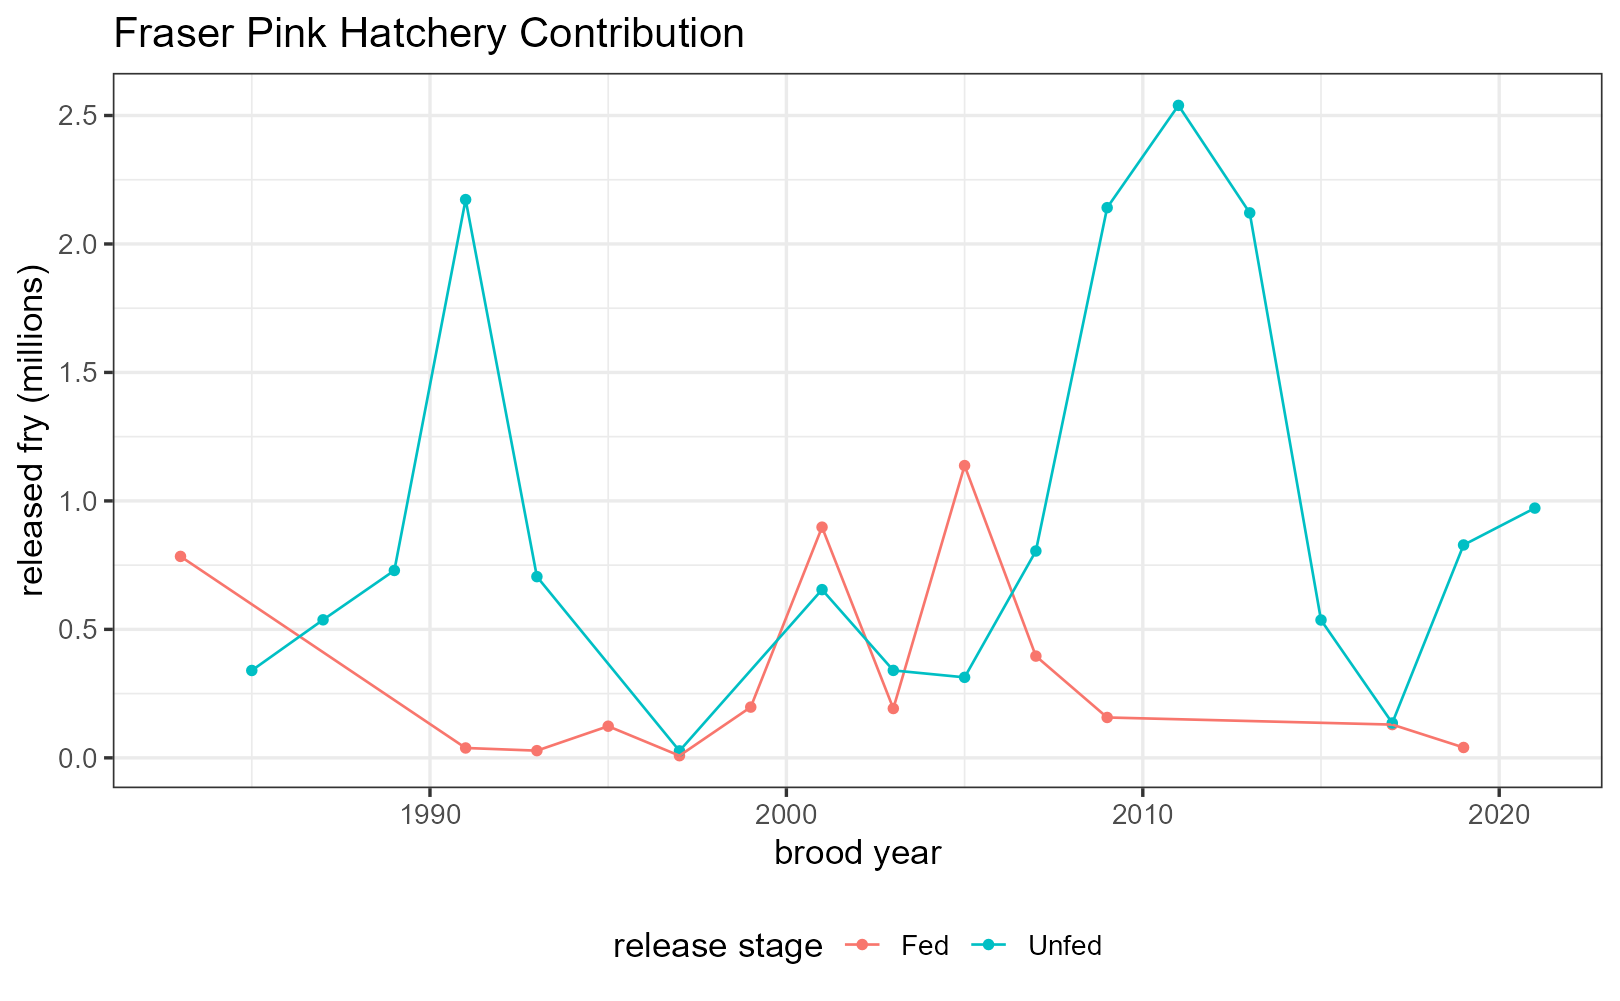
\includegraphics[width=6in]{figure/hatchery-influence}}{Figure \ref{fig:fig-hatch-cont}} 

}

\caption{Number of Pink Fry released on the Fraser. Data only includes releases of fish that were manually stripped of eggs and eggs placed in holding boxes (i.e.~does not include progeny of fish that naturally spawned in constructed spawning channels near hatcheries).}\label{fig:fig-hatch-cont}
\end{figure}

\begin{figure}[htb]

{\centering \pdftooltip{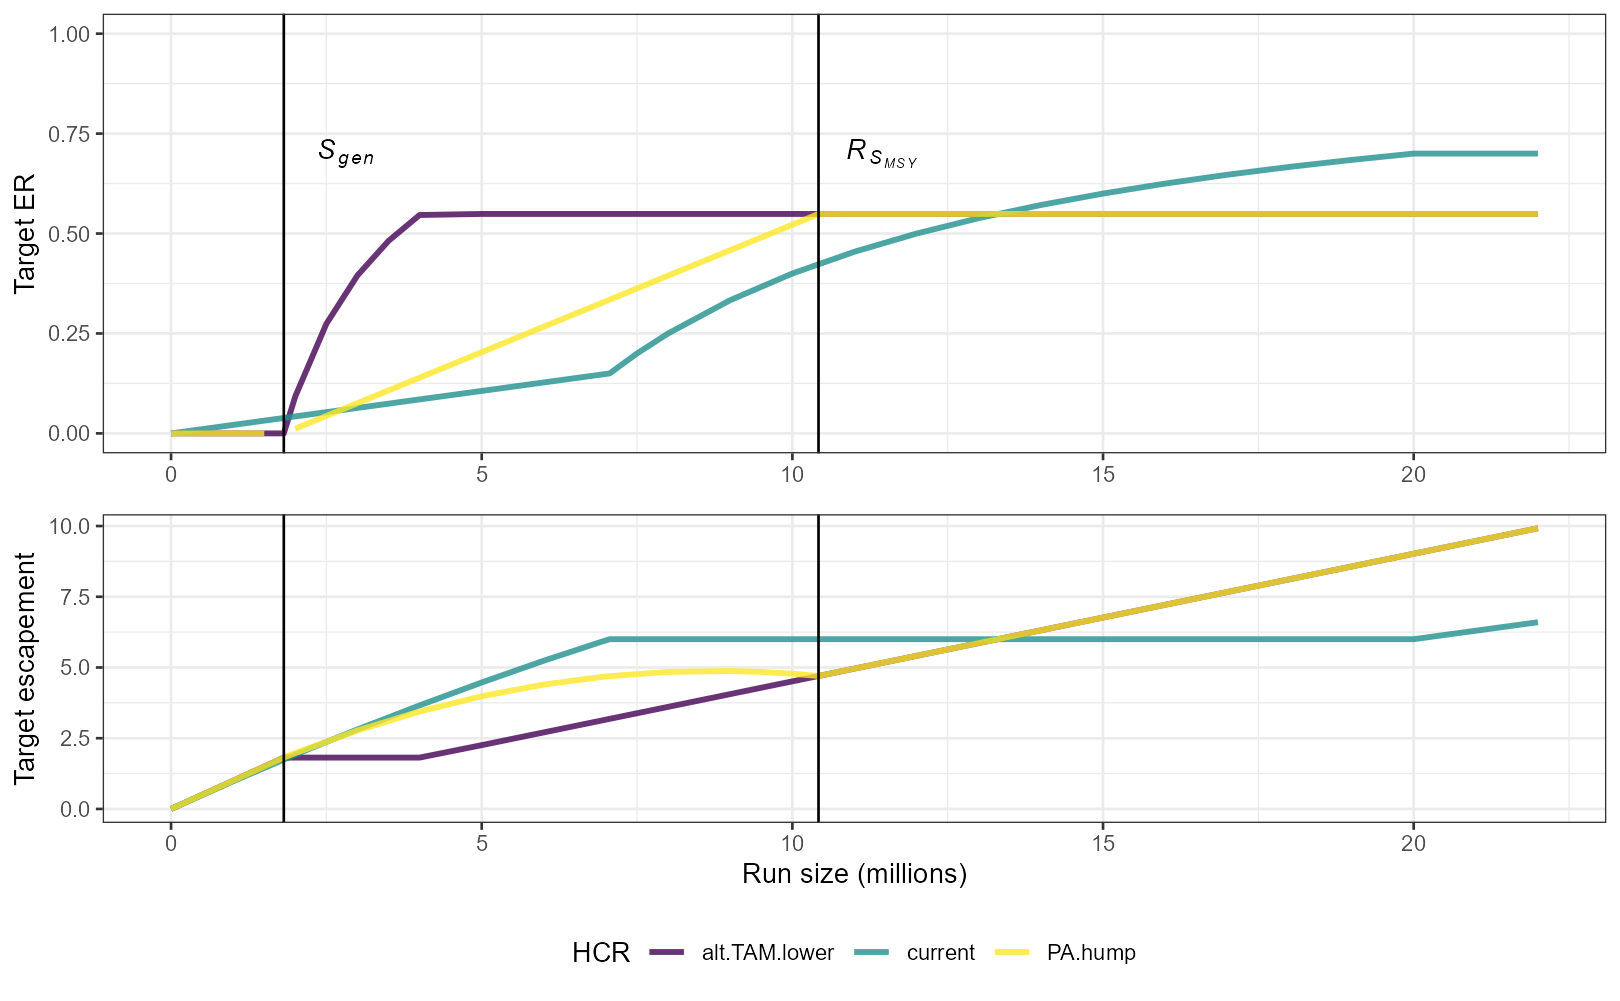
\includegraphics[width=6in]{figure/HCRs}}{Figure \ref{fig:fig-HCRs}} 

}

\caption{Current and alternative (PA alternate) harvest control rules (HCRs). The top panel is the HCR relating target catch to run-size while the bottom panel illustrates the resulting target escapement as a function of run-size. Vertical lines denote Limit (\(S_{GEN}\)) and Upper Stock (80\%\(S_{MSY}\)) reference points, in run-size units.}\label{fig:fig-HCRs}
\end{figure}

\begin{figure}[htb]

{\centering \pdftooltip{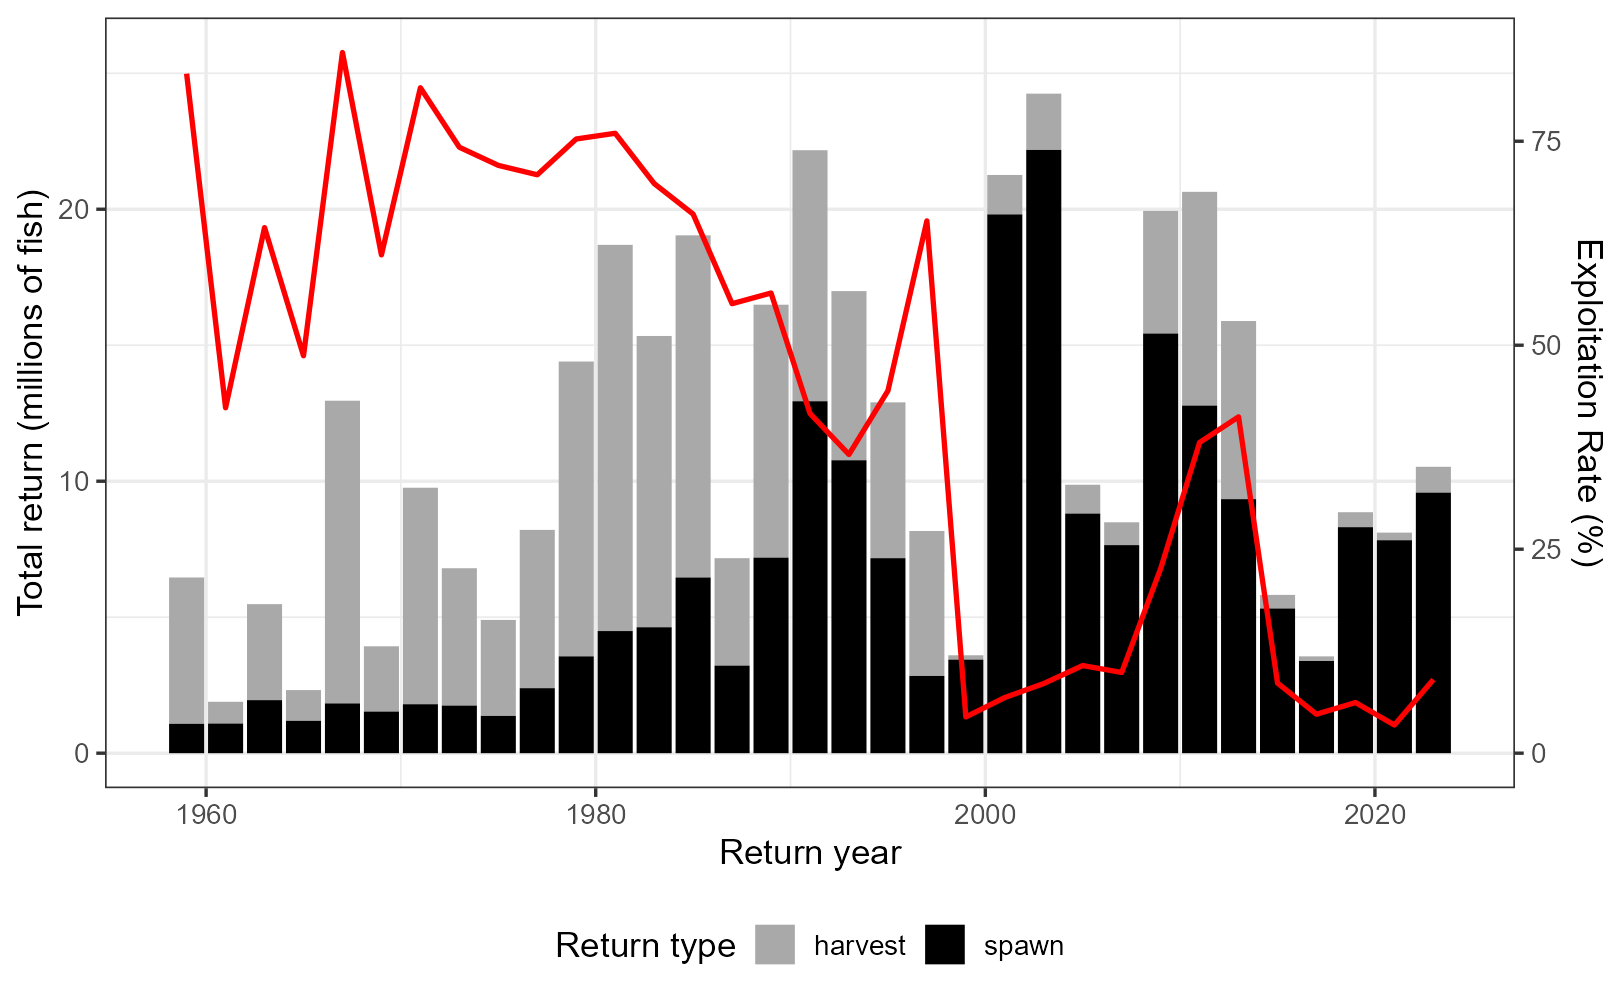
\includegraphics[width=6in]{figure/catch-esc}}{Figure \ref{fig:fig-catch-esc}} 

}

\caption{Spawning escapement and catch from 1959 to present. Resulting exploitation rate is show in red on secondary y-axis.}\label{fig:fig-catch-esc}
\end{figure}

\begin{figure}[htb]

{\centering \pdftooltip{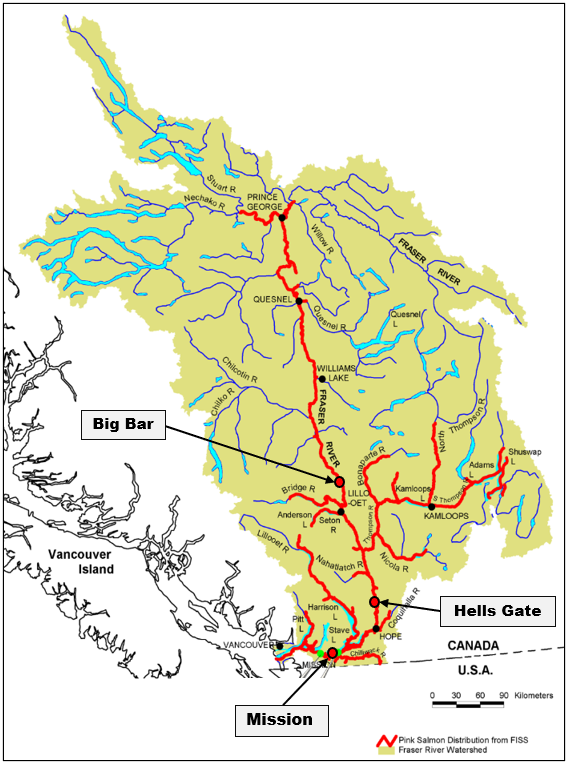
\includegraphics[width=6in]{figure/map}}{Figure \ref{fig:fig-map}} 

}

\caption{Fraser River Basin, extent of Pink Salmon spawning distribution (red), and approximate locations of the Mission hydroacoustics site, Hells Gate and Big Bar. Map adapted from (\protect\hyperlink{ref-grantFraserRiverPink2014}{Grant et al. 2014}).}\label{fig:fig-map}
\end{figure}

\begin{figure}[htb]

{\centering \pdftooltip{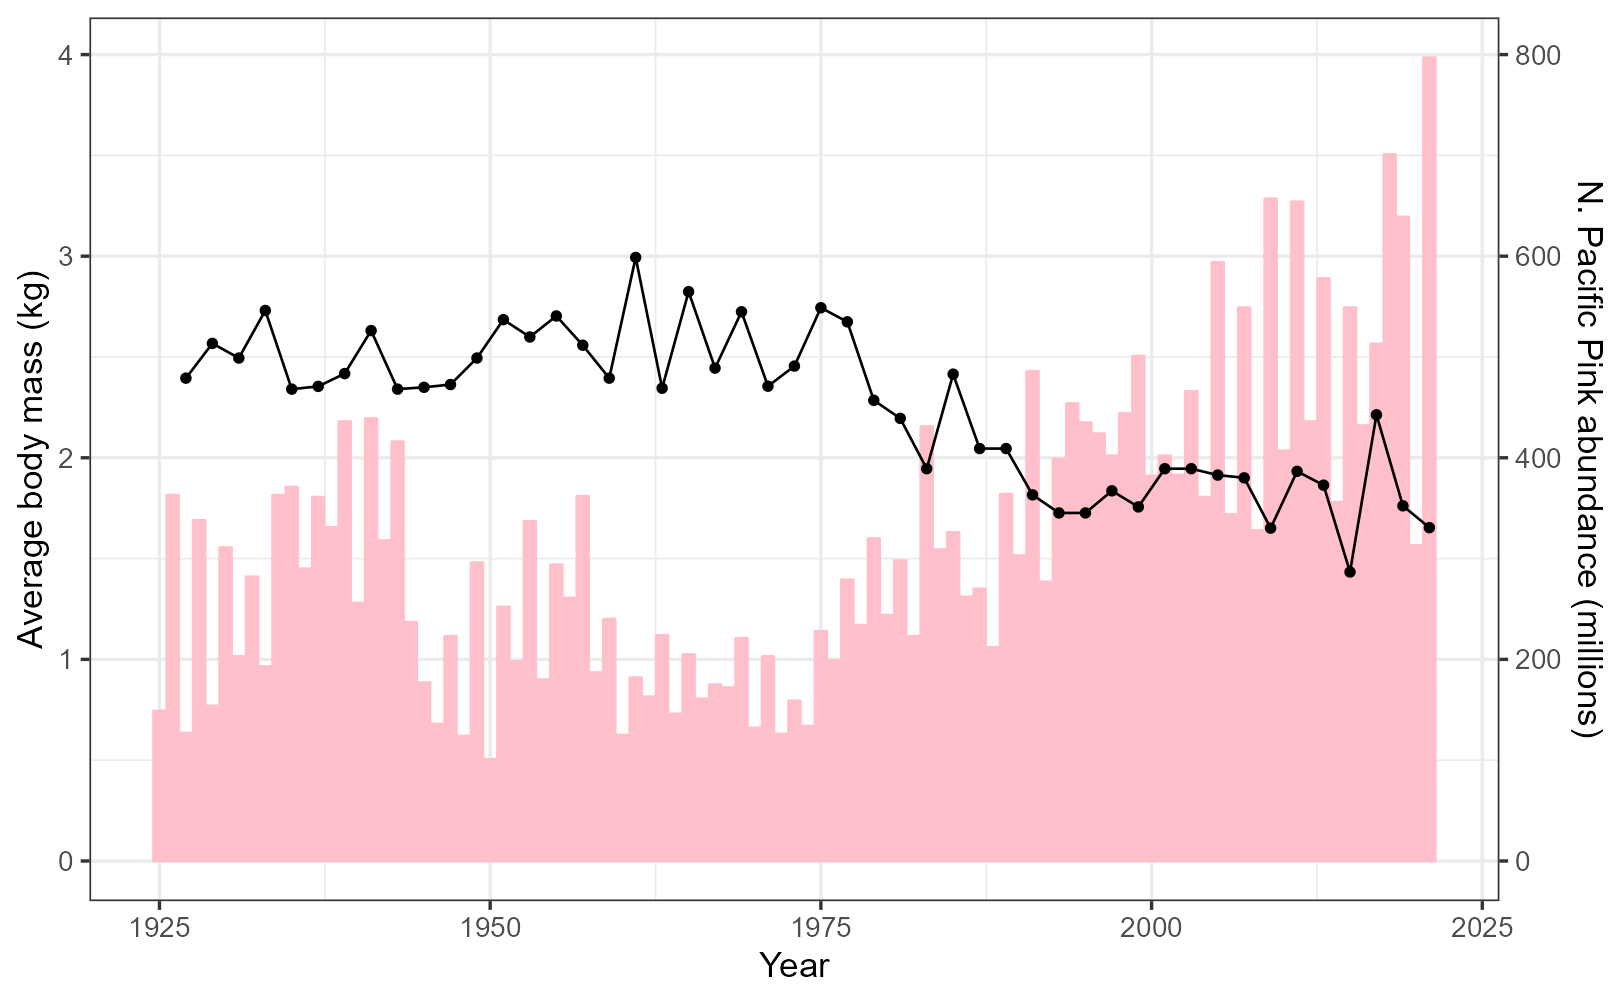
\includegraphics[width=6in]{figure/avg-mass}}{Figure \ref{fig:fig-avg-mass}} 

}

\caption{Average body mass (kg) for Fraser Pinks over time and total returns of Pink Salmon across the North Pacific, 1925-present. Body mass data were taken from Pacific Salmon Commission (\protect\hyperlink{ref-pacificsalmoncommissionPSCBiologicalData2023}{2023}) and time series of North Pacific wide Pink Salmon abundance are from (\protect\hyperlink{ref-ruggeroneNumbersBiomassNatural2018}{Ruggerone and Irvine 2018}) and updated through present.}\label{fig:fig-avg-mass}
\end{figure}

\begin{figure}[htb]

{\centering \pdftooltip{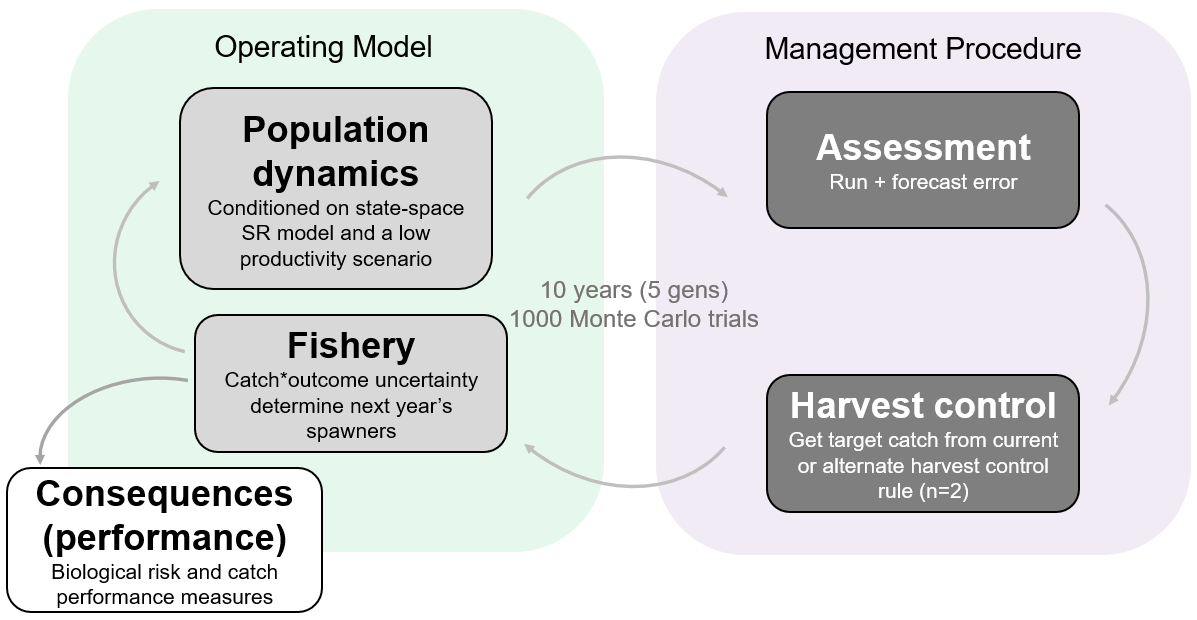
\includegraphics[width=6in]{figure/fwd-sim-schematic}}{Figure \ref{fig:fig-schematic}} 

}

\caption{Illustration of steps in the forward simulation highlighting alternate scenarios in population dynamics and harvest control rules.}\label{fig:fig-schematic}
\end{figure}

\begin{figure}[htb]

{\centering \pdftooltip{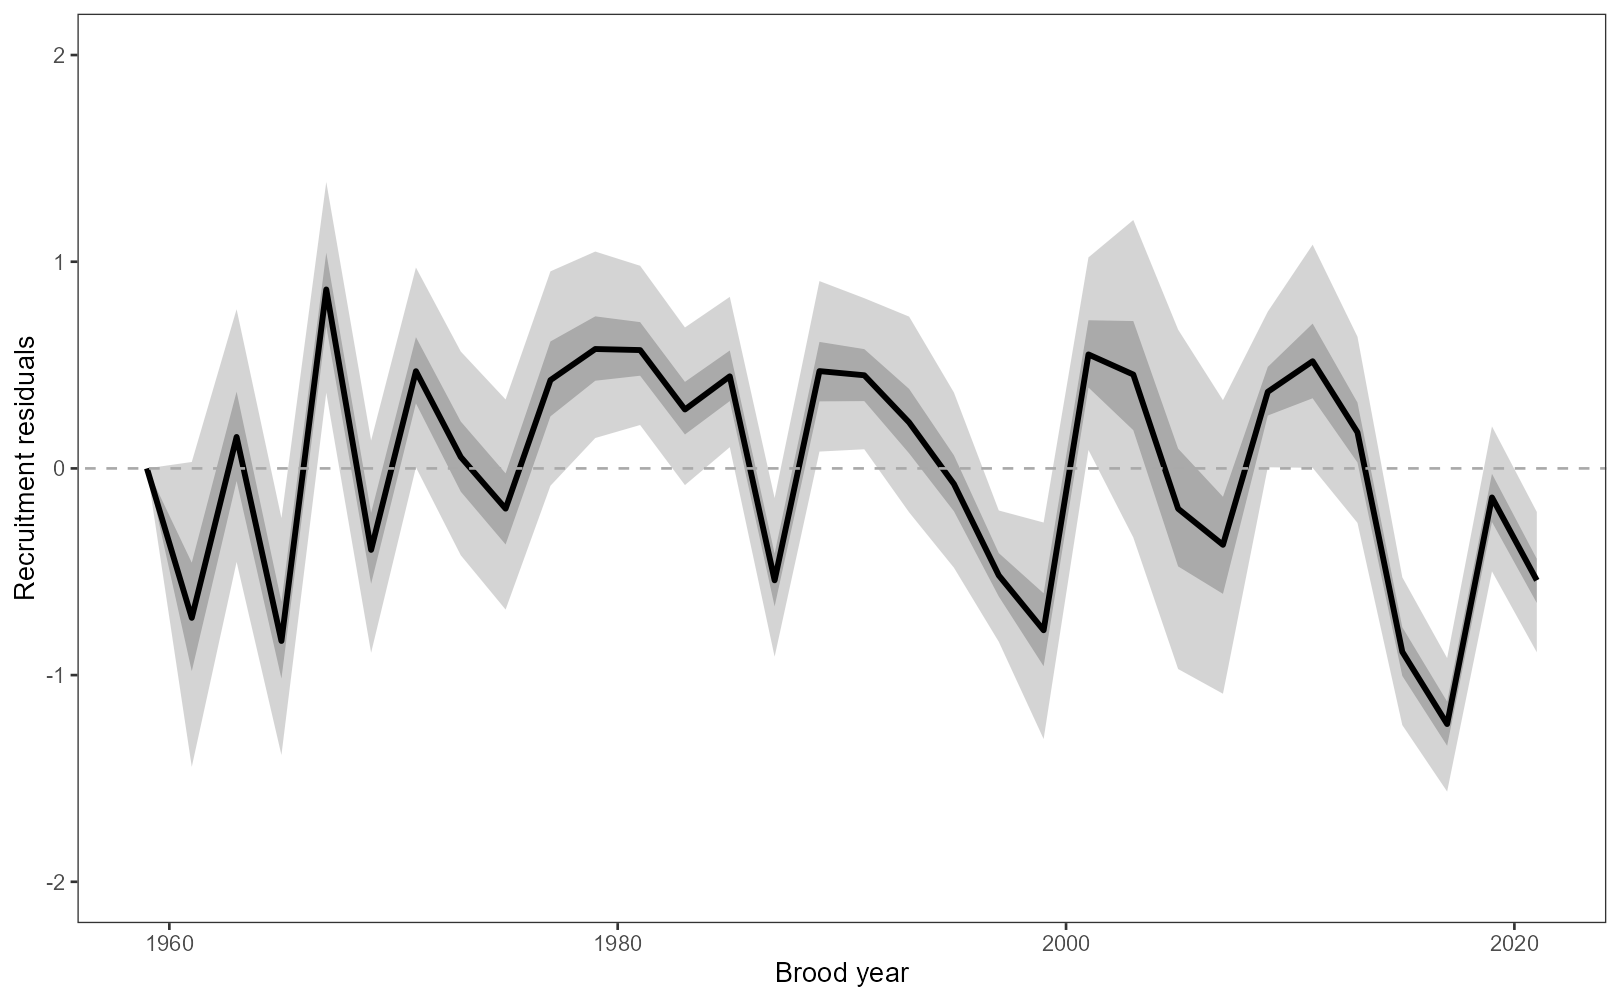
\includegraphics[width=6in]{figure/rec-resid}}{Figure \ref{fig:fig-rec-resid}} 

}

\caption{Recruitment residuals from the Fraser Pink spawner-recruitment relationship over time. Thick black line is the median estimates while the shaded band is the 80th percentile.}\label{fig:fig-rec-resid}
\end{figure}

\begin{figure}[htb]

{\centering \pdftooltip{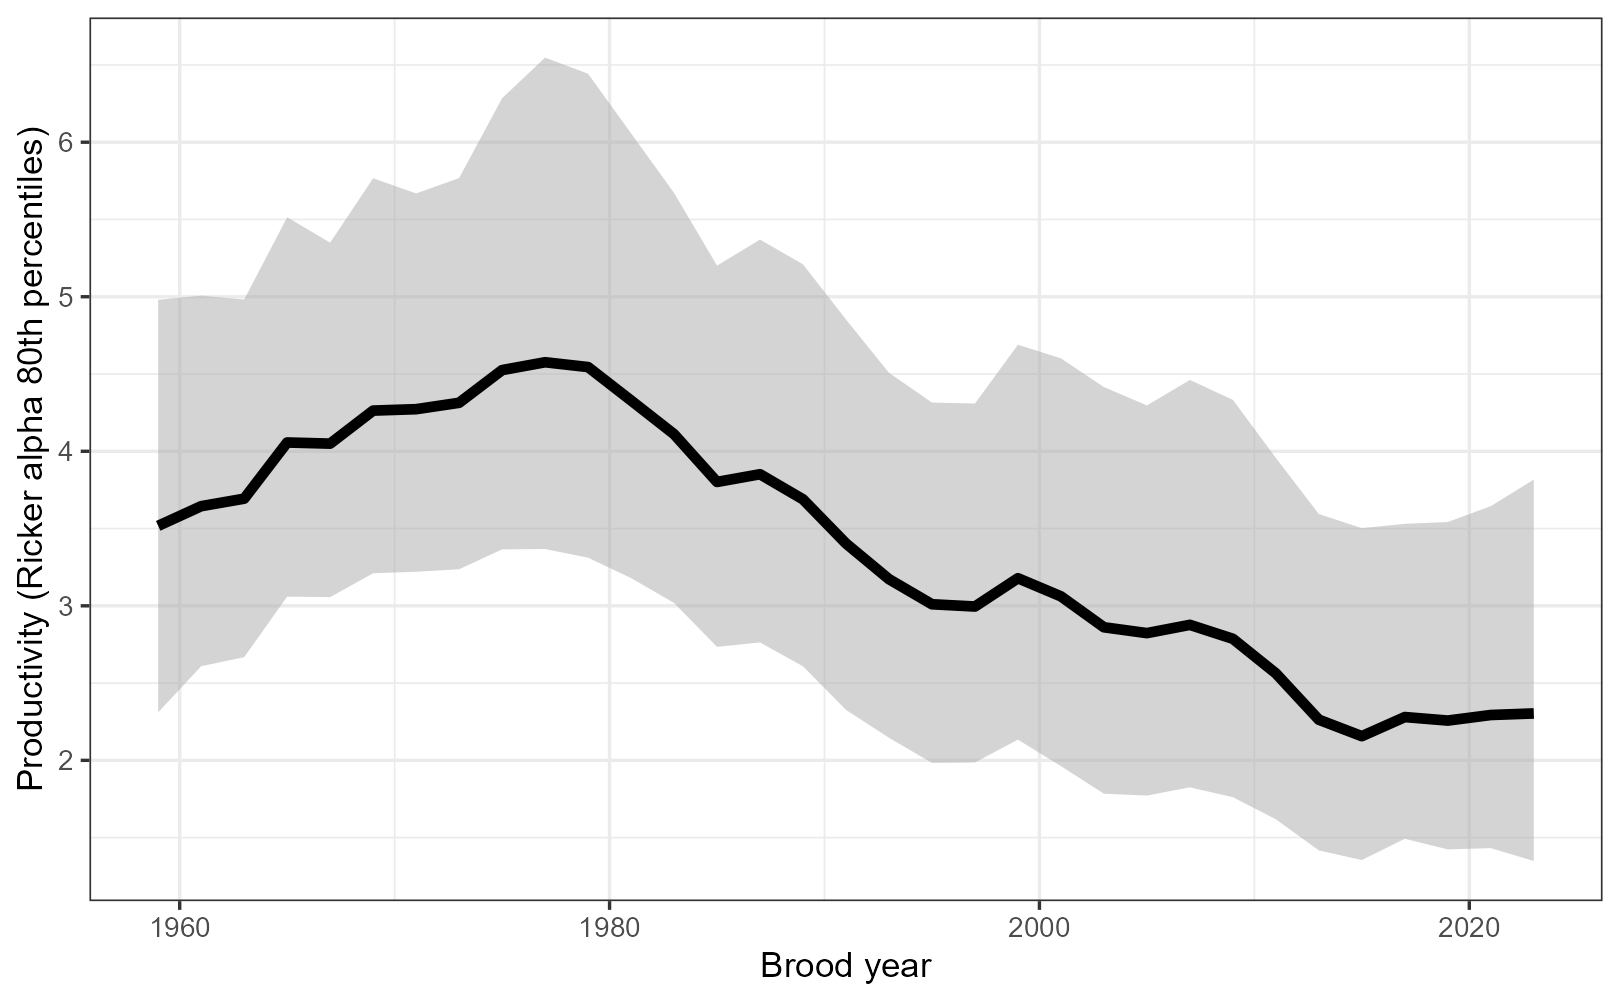
\includegraphics[width=6in]{figure/tv-alpha}}{Figure \ref{fig:fig-tv-alpha}} 

}

\caption{Time-varying productivity (Ricker \(\alpha\) parameter) fit from the model used to project population dynamics forward in the closed-loop simulation.}\label{fig:fig-tv-alpha}
\end{figure}

\begin{figure}[htb]

{\centering \pdftooltip{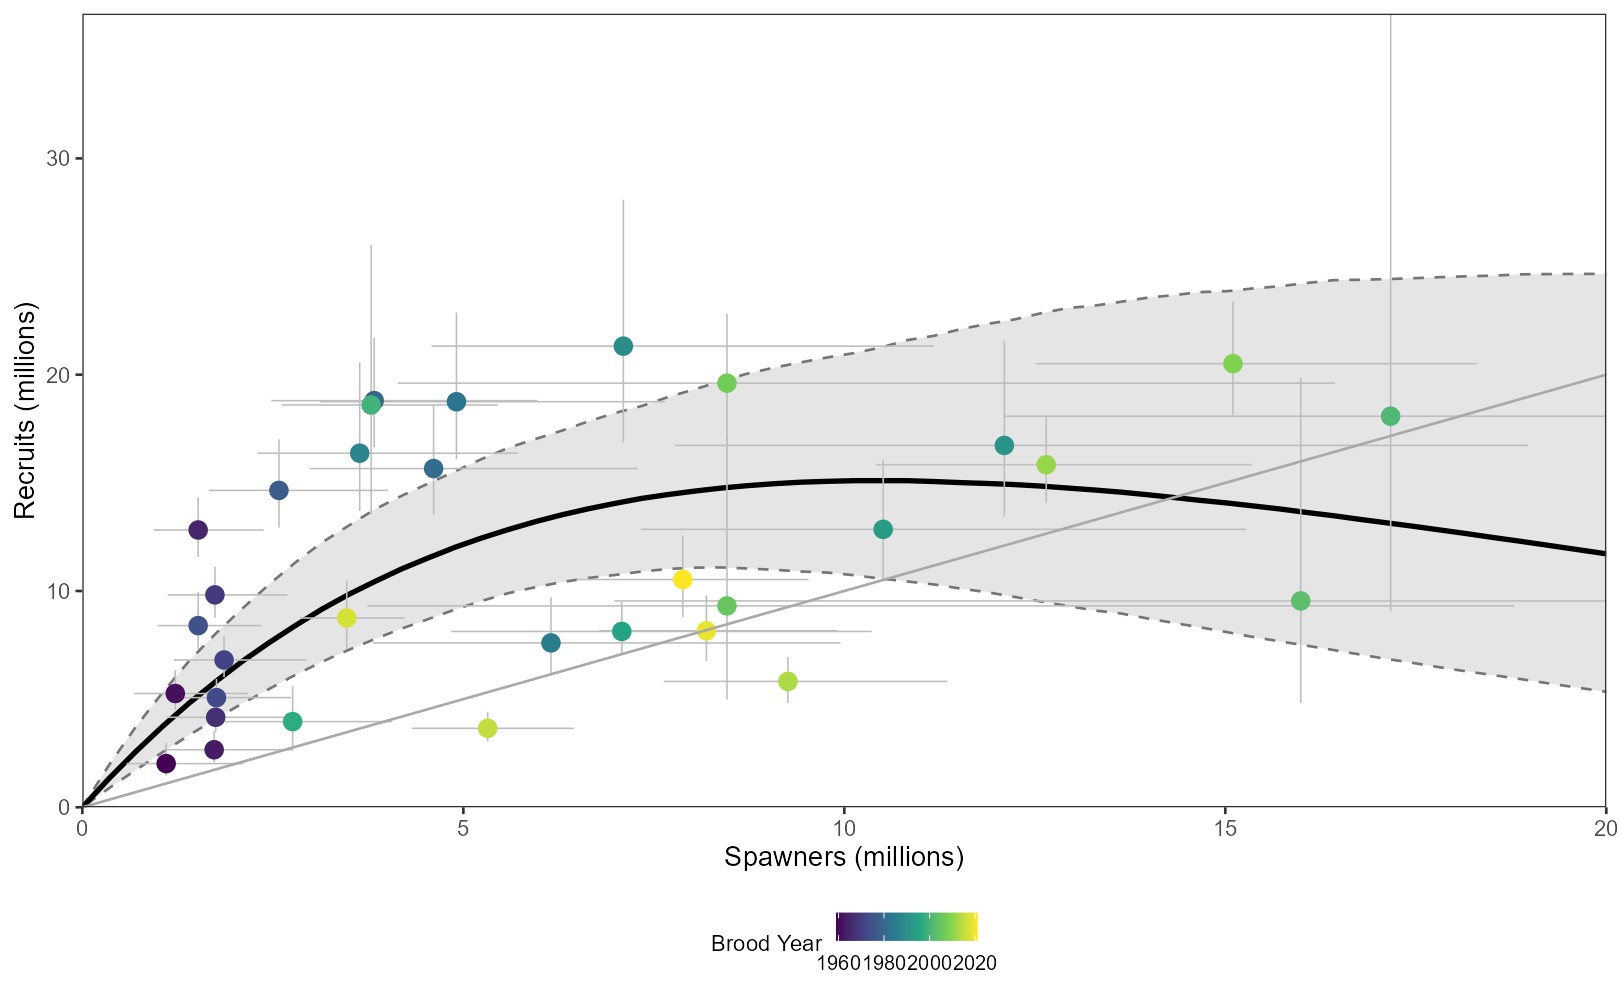
\includegraphics[width=6in]{figure/SRR}}{Figure \ref{fig:fig-SRR}} 

}

\caption{Fraser Pink Salmon spawner-recruitment relationship. Error bars around points, which are colour coded by brood year, and relationship are 80\% credible interval while the thick black line is the expected relationship.}\label{fig:fig-SRR}
\end{figure}

\begin{figure}[htb]

{\centering \pdftooltip{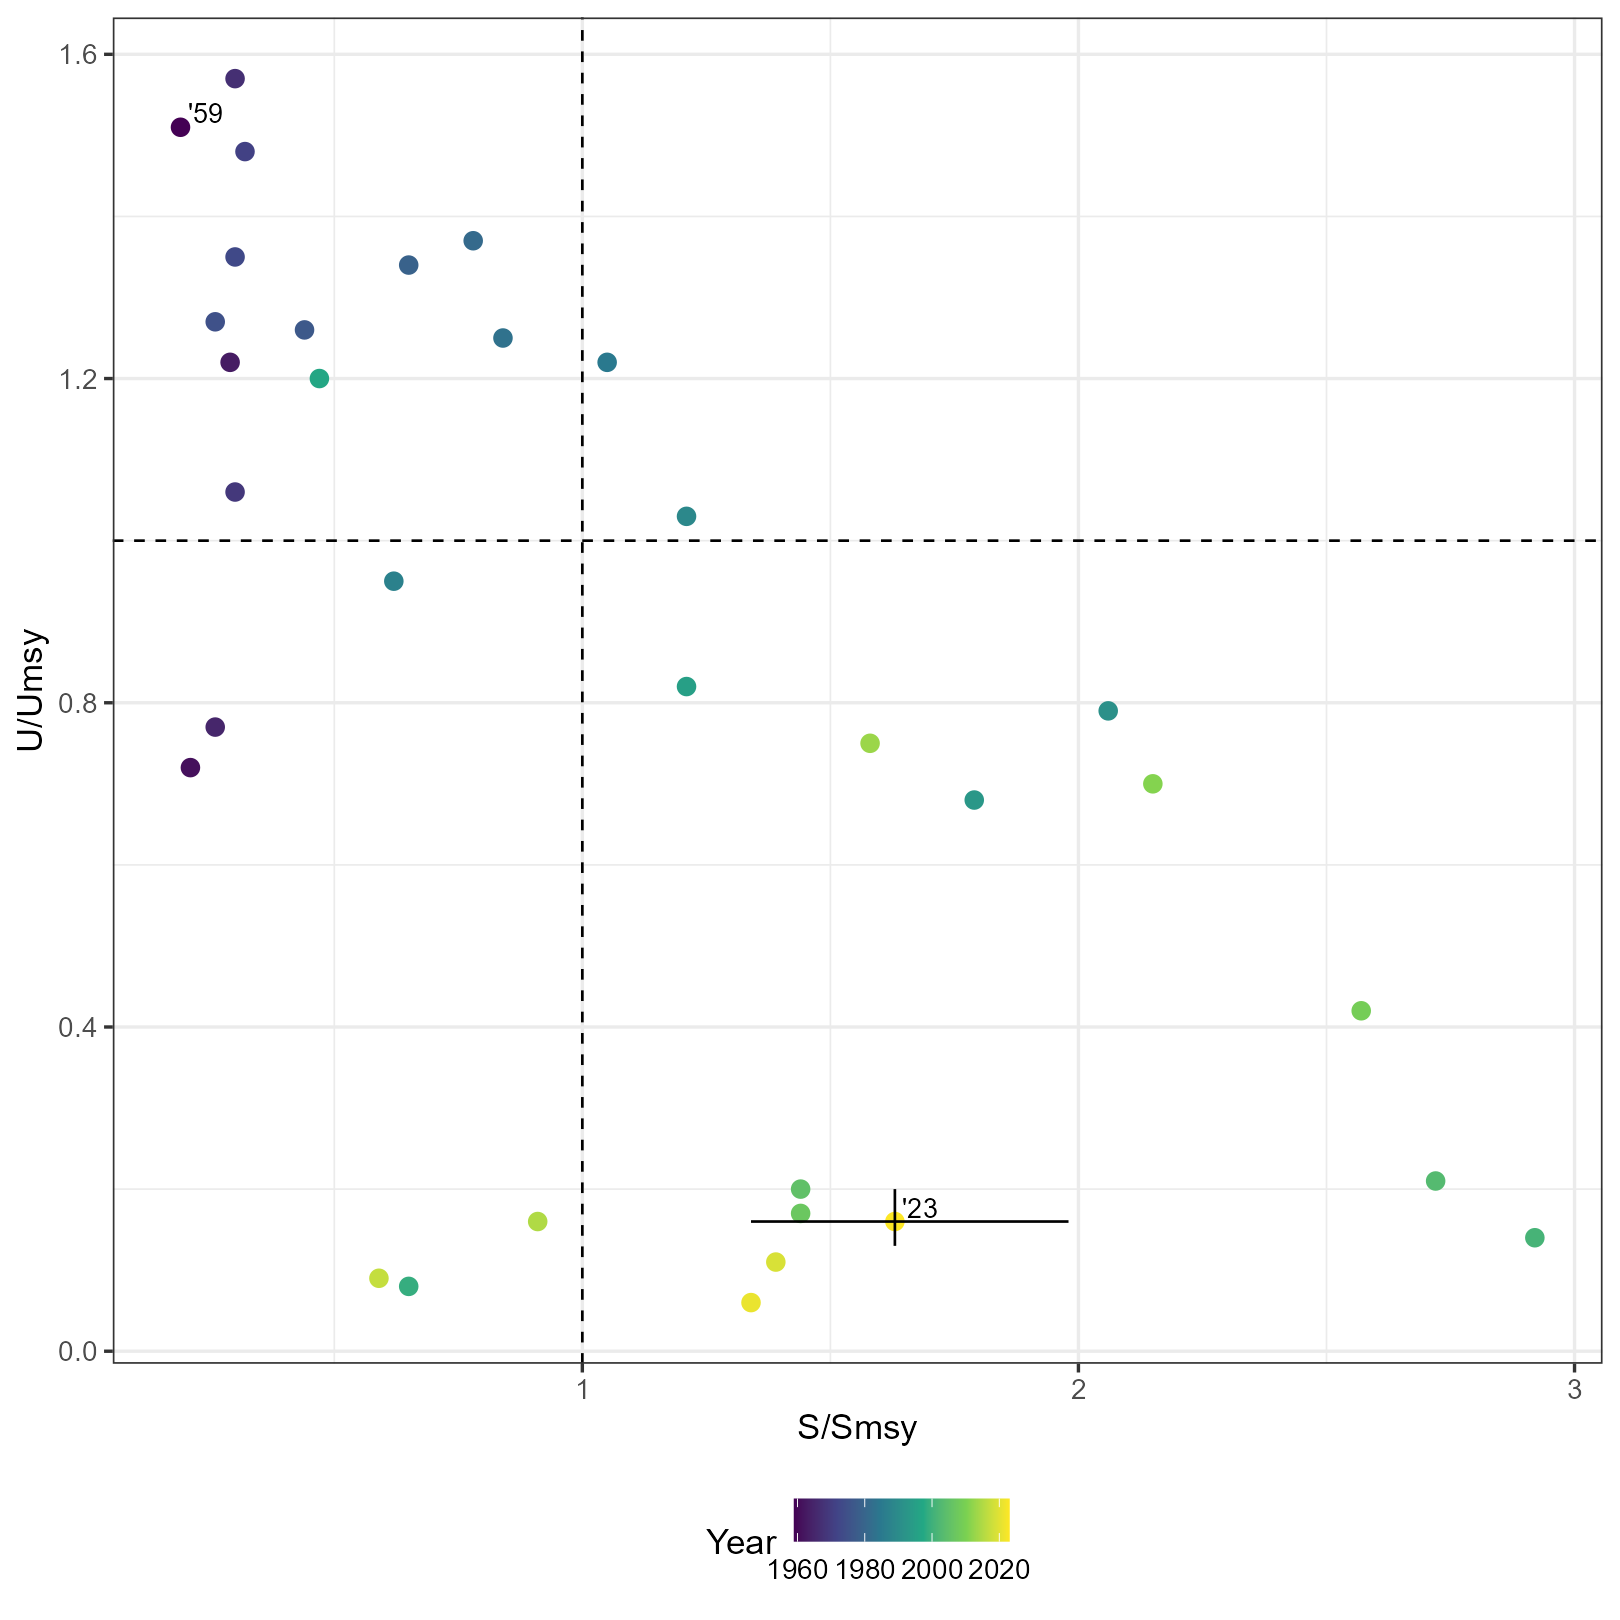
\includegraphics[width=6in]{figure/kobe}}{Figure \ref{fig:fig-kobe}} 

}

\caption{Kobe plot of Fraser Pink status overtime. Years are colour coded and the first and last ones are labelled. 80\% credible intervals are included for the last year of assessment.}\label{fig:fig-kobe}
\end{figure}

\begin{figure}[htb]

{\centering \pdftooltip{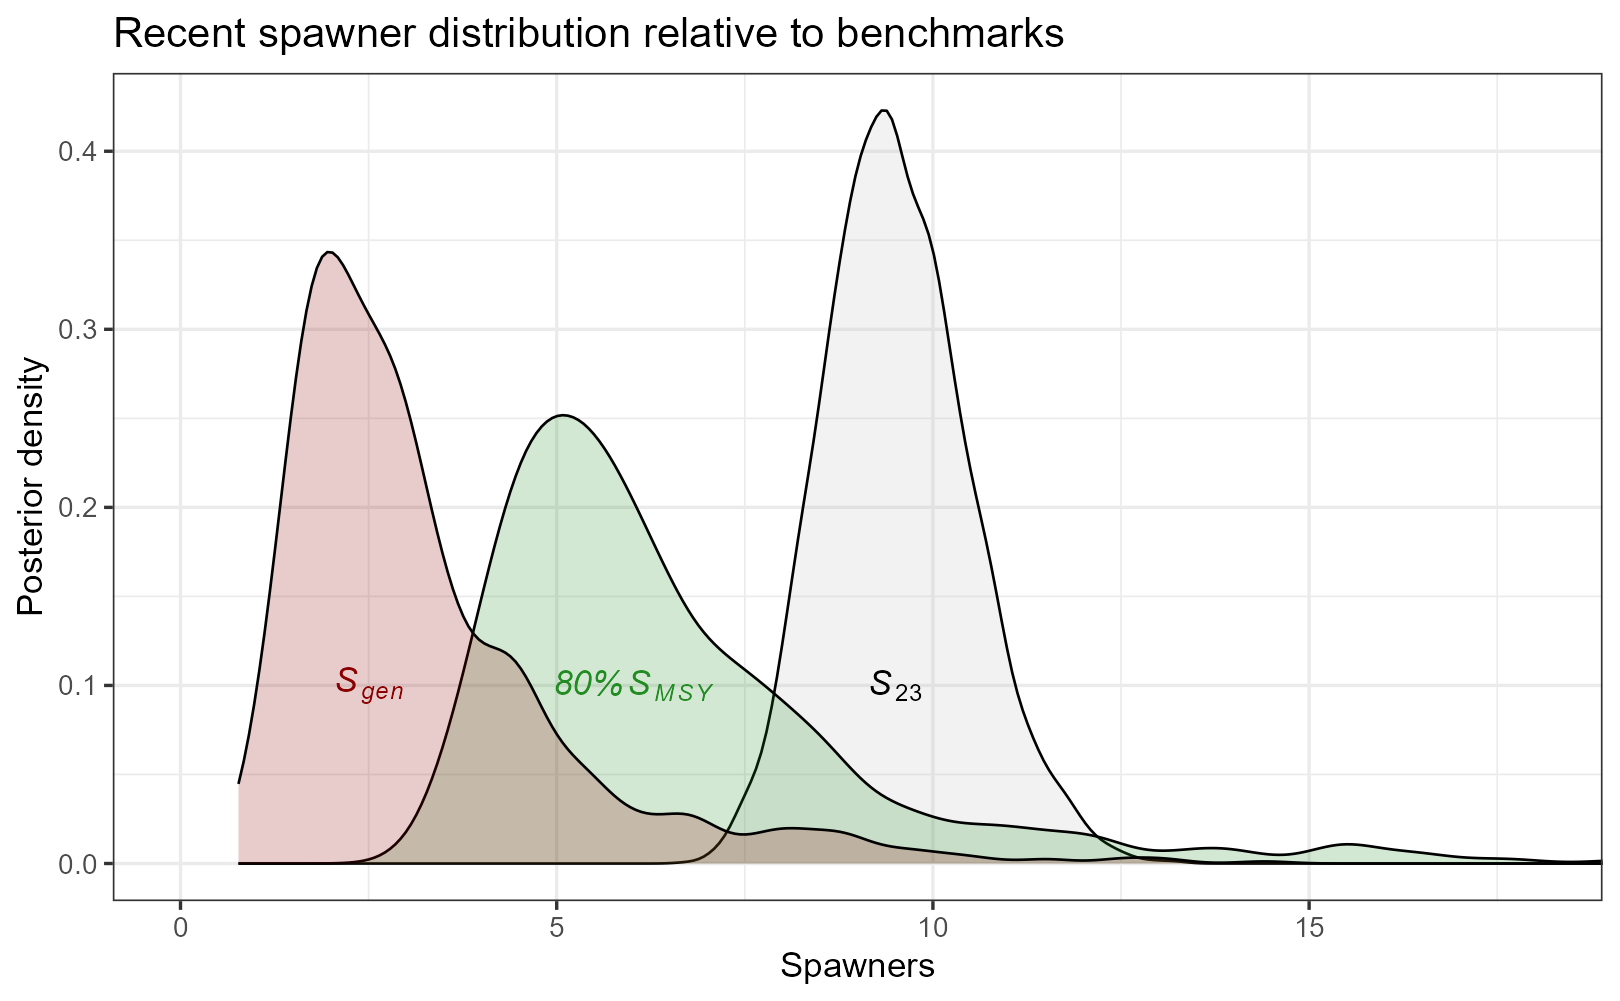
\includegraphics[width=6in]{figure/recent-status}}{Figure \ref{fig:fig-status}} 

}

\caption{Posterior distributions of candidate reference points \(S_{gen}\), the LRP (red), \(S_{MSY}\), the USR (green) and the latent state of spawners in the most recent generation (2023, black).}\label{fig:fig-status}
\end{figure}

\begin{figure}[htb]

{\centering \pdftooltip{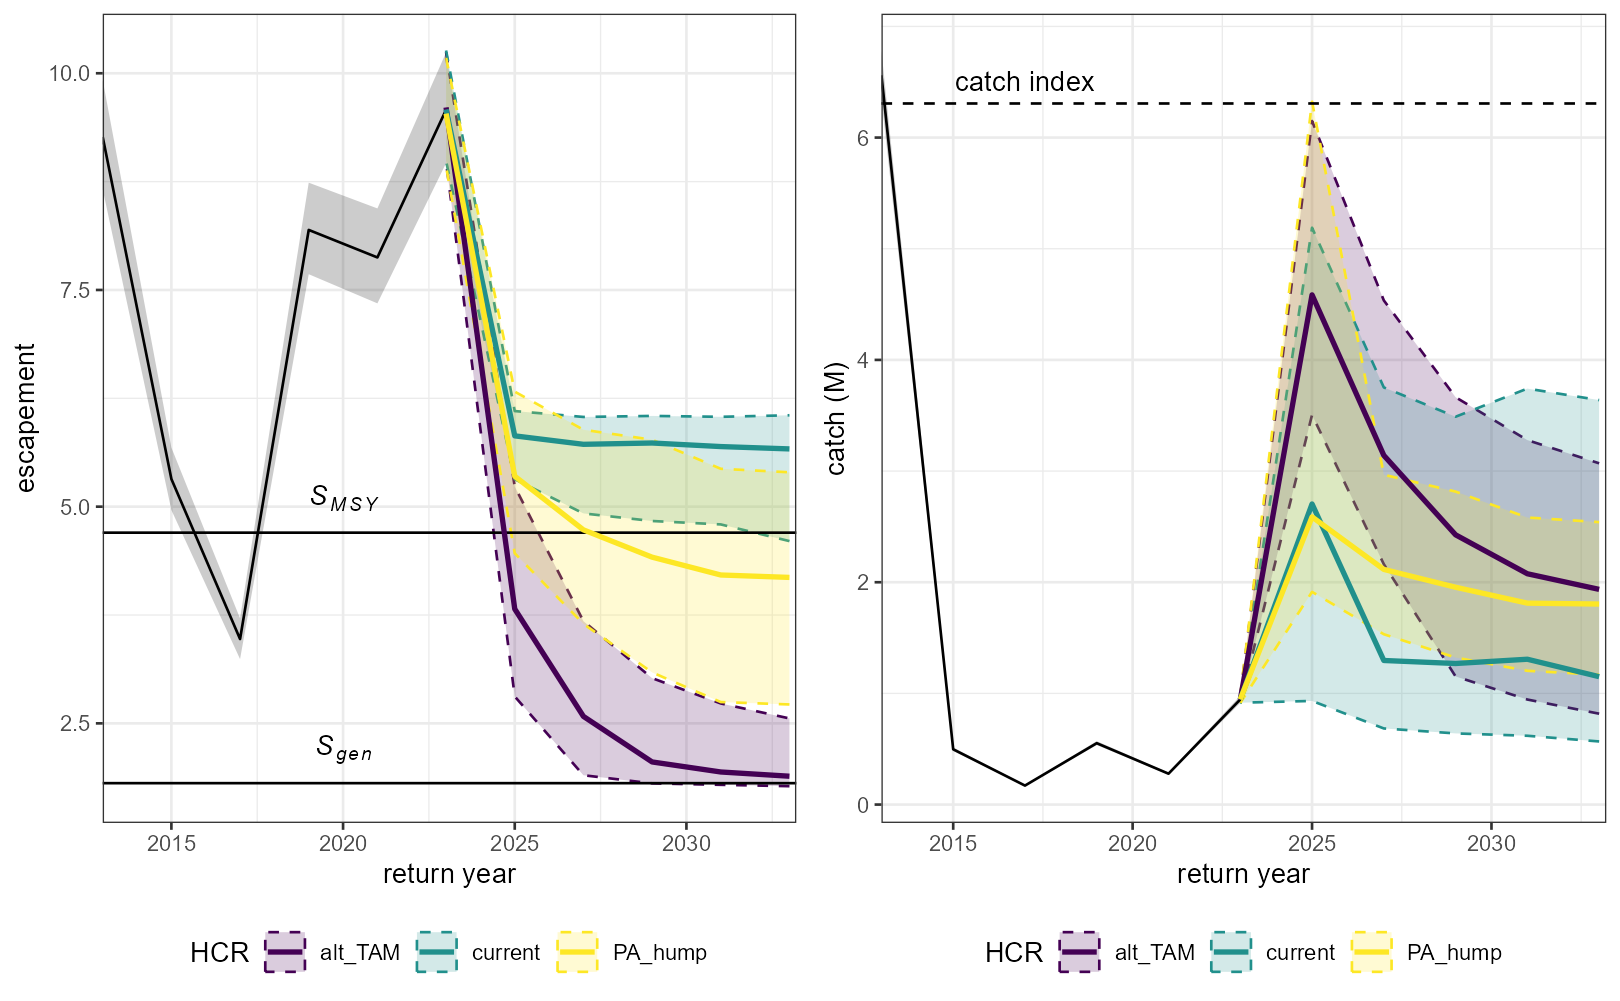
\includegraphics[width=6in]{figure/fwd-SC}}{Figure \ref{fig:fig-fwd-SC}} 

}

\caption{Projected Fraser Pink spawners and catch (both in millions of fish; shaded and coloured lines) over next 10 years when either the current or alternative illustrative HCRs are applied. Historical escapement and catch (black) are included for reference. Shaded polygons are 80\% credible intervals and solid lines are medians. The catch index in right hand panel is defined as the average of the top 3 years of catch from 2001 to present.}\label{fig:fig-fwd-SC}
\end{figure}
\clearpage

\hypertarget{tables}{%
\section{TABLES}\label{tables}}


\begin{longtable}[t]{l>{\raggedright\arraybackslash}p{8cm}l} \caption{\label{tab:tab-spawner-est-methods}Summary of changes in methods used to assess spawning escapement over time and assumed coefficients of variation (CVs) for each period which were used to define magnitude of observation error in state-space spawner-recruitment model.}\\ \toprule Years & Assessment Method & CV\\ \midrule \endfirsthead \multicolumn{3}{l}{\textit{... Continued from previous page}} \\ \hline \caption*{}\\ \toprule Years & Assessment Method & CV\\ \midrule \endhead \hline \multicolumn{3}{l}{\textit{Continued on next page ...}} \\ \endfoot \bottomrule \endlastfoot 1957-61 & Early International Pacific Salmon Fishing Commission (IPSFC, currently known as the Pacific Salmon Commission, PSC) system specific mark-recapture: low tagging effort & 35\%\\ 1963-91 & IPSFC ('63-'85) and DFO ('87-'91) system specific mark-recapture: high precision methods in larger systems (90\% of stock) and lower precision in the remainder & 25\%\\ 1993-01 & DFO mainstem mark-recapture assessment downstream of major spawning grounds & 20\%\\ 2003-07 & PSC test fishery: escapement derived from seine boats in marine and catch data & 50\%\\ 2009-present & PSC Mission sonar & 10\%\\* \end{longtable}

\clearpage


\begin{longtable}[t]{l>{\raggedright\arraybackslash}p{6.5cm}c} \caption{\label{tab:tab-perf-metrics-descriptions}Biological and fishery performance measures used in the closed-loop simulations to assess HCR performance.}\\ \toprule Metric & Description & Equation\\ \midrule \endfirsthead \multicolumn{3}{l}{\textit{... Continued from previous page}} \\ \hline \caption*{}\\ \toprule Metric & Description & Equation\\ \midrule \endhead \hline \multicolumn{3}{l}{\textit{Continued on next page ...}} \\ \endfoot \bottomrule \endlastfoot \% replicate simulations < LRP & Probability the stock spawner abundance falls below the Limit Reference Point across replicate simulations and years, where $n$ rep is the number of replicate simulations and $t_1$ and $t_2$ are the first and last years over which the metric is calculated & $\frac{\sum_{\substack{n_{rep}\\s =1}}\sum_{\substack{t_1\\s   _2}}S_t<S_{gen}} {t_2-t_1+1}$\\ \% replicate simulations > USR & Probability the stock spawner abundance falls above the Upper Stock Reference Point across replicate simulations and years & $\frac{\sum_{\substack{n_{rep}\\s =1}}\sum_{\substack{t_1\\s  _2}}S_t>0.8S_{MSY}} {t_2-t_1+1}$\\ average annual catch & Average catch across replicate simulations and years & $\frac{\sum_{\substack{n_{rep}\\s =1}}\sum_{\substack{t_1\\s   _2}}S_tC_t} {t_2-t_1+1}$\\ catch stability (1/CV) & Stability in average catch across replicate simulations and years($\mu_C$), where is $\sigma_C$ the standard deviation in catch & $\cfrac{1}{\tfrac{\sigma_C}{\mu_C}}$\\ relative catch metric & Probability annual catch is greater than the average of the top 3 years of catch since 2000 ($C_{top}$), a semi-arbitrary indicator of a ‘good year’ & $\frac{\sum_{\substack{n_{rep}\\s =1}}\sum_{\substack{t_1\\s    _2}}C_t>C_{top}} {t_2-t_1+1}$\\* \end{longtable}

\clearpage


\begin{longtable}[t]{l>{\raggedright\arraybackslash}p{6cm}l>{\raggedright\arraybackslash}p{5cm}} \caption{\label{tab:tab-priors}Prior probability distributions for parameters.}\\ \toprule Parameter & Prior & Bounds & Description\\ \midrule \endfirsthead \multicolumn{4}{l}{\textit{... Continued from previous page}} \\ \hline \caption*{}\\ \toprule Parameter & Prior & Bounds & Description\\ \midrule \endhead \hline \multicolumn{4}{l}{\textit{Continued on next page ...}} \\ \endfoot \bottomrule \endlastfoot $ln(\alpha)$ & $\sim N(1,2)$ & $[0,\inf]$ & Natural log of intrinsic rate of growth.\\ $ln(\beta)$ & $\sim N\bigg(ln(1/S_{MAX}) - 0.5\sigma_{S_{MAX}}^2,                                    \sqrt{ln(1+ \cfrac{(\cfrac{1}{\sigma S_{MAX}})^2}{(\cfrac{1}{S_{MAX}})^2}})\biggr)$ &  & Magnitude of within brood-year density-dependence, where $S_{MAX}$ is the maximum spawner abundance times 0.75.\\ $\phi$ & $\sim U(-1,1)$ & $[-1,1]$ & Lag-one correlation in interannual variation in survival.\\ $\sigma_R$ & $\sim N(1,2)$ & $[0,\inf]$ & White noise process standard deviation in survival.\\ $ln(R_0)$ & $\sim N(0,20)$ & $[0,\inf]$ & Natural log of unobserved recruitment in the first year of process model.\\ $\sigma_{R_0}$ & $\sim Inv-Gamma(2,1)$ & $[0,\inf]$ & Standard deviation in unobserved recruitment in the first year of process model.\\* \end{longtable}

\clearpage


\begin{longtable}[]{@{}llccclc@{}}
\caption{\label{tab:tab-bench-parms}Posterior means, medians and credible intervals for leading spawner-recruitment parameters and associated biological reference points. Also shown are estimates of the effective sample size (\(N_{eff}\)) and potential scale reduction factor (\(\hat{R}\)) for parameters estimated by the model.}\tabularnewline
\toprule\noalign{}
& Median & 10th percentile & 90th percentile & Mean & \(N_{eff}\) & \(\hat{R}\) \\
\midrule\noalign{}
\endfirsthead
\toprule\noalign{}
& Median & 10th percentile & 90th percentile & Mean & \(N_{eff}\) & \(\hat{R}\) \\
\midrule\noalign{}
\endhead
\bottomrule\noalign{}
\endlastfoot
\(S_{gen}\) & 1.72 & 1.10 & 2.70 & 1.91 & & \\
80\% \(S_{MSY}\) & 4.60 & 3.64 & 6.11 & 4.86 & & \\
\(U_{MSY}\) & 0.56 & 0.47 & 0.63 & 0.56 & & \\
\(S_{eq}\) & 14.10 & 11.41 & 18.48 & 14.90 & & \\
\(\alpha\) & 3.94 & 3.02 & 5.02 & 1.36 & 2891 & 1.0006 \\
\(\beta\) & 0.59 & 0.49 & 0.73 & 0.10 & 2769 & 1.0004 \\
\(\phi\) & 0.10 & 0.06 & 0.13 & 0.09 & 1574 & 1.0002 \\
\(\sigma_{R}\) & 0.06 & -0.09 & 0.31 & 1.09 & 3278 & 0.9992 \\
\end{longtable}

\begin{longtable}[t]{>{\raggedright\arraybackslash}p{1.5cm}>{\raggedright\arraybackslash}p{1.5cm}>{\centering\arraybackslash}p{1.5cm}>{\centering\arraybackslash}p{1.5cm}>{\centering\arraybackslash}p{3cm}>{\centering\arraybackslash}p{3cm}>{\centering\arraybackslash}p{1.5cm}} \caption{\label{tab:tab-HCR-performance}Biological and fishery performance of current and alternative illustrative HCR for both baseline and robustness test operating model scenarios.}\\ \toprule HCR & Scenario & \% below $S_{gen}$ & \% above $S_{MSY}$ & Median annual catch & Catch stability & \% above catch index\\ \midrule \endfirsthead \multicolumn{7}{l}{\textit{... Continued from previous page}} \\ \hline \caption*{}\\ \toprule HCR & Scenario & \% below $S_{gen}$ & \% above $S_{MSY}$ & Median annual catch & Catch stability & \% above catch index\\ \midrule \endhead \hline \multicolumn{7}{l}{\textit{Continued on next page ...}} \\ \endfoot \bottomrule \endlastfoot base & current & 4.28 & 87.54 & 10.3 (2.47-22.16) & 1.21 (0.35-2.38) & 64.3\\ base & PA alt & 5.16 & 87.46 & 8.84 (2.62-18.38) & 1.38 (0.48-2.8) & 66.62\\ base & no fishing & 3.96 & 93.14 & 0 (0-0) & NA & 0\\ low prod & current & 9.4 & 73.48 & 3.44 (0.49-11.69) & 0.73 (0.14-1.78) & 35.8\\ low prod & PA alt & 20.18 & 63.7 & 2.82 (1.14-10.73) & 1.1 (0.36-2.57) & 37.32\\ low prod & no fishing & 5.82 & 89.42 & 0 (0-0) & NA & 0\\* \end{longtable}

\clearpage

\hypertarget{references}{%
\section{REFERENCES CITED}\label{references}}

% This manually sets the header for this unnumbered chapter.
\noindent
\vspace{-2em}
\setlength{\parindent}{-0.2in}
\setlength{\leftskip}{0.2in}
\setlength{\parskip}{8pt}

\hypertarget{refs}{}
\begin{CSLReferences}{1}{0}
\leavevmode{\hypertarget{ref-adkisonReviewSalmonSpawnerRecruitment2021}{}}%
Adkison, M.D. 2021. \link{https://doi.org/gpdfdc}{A {Review} of {Salmon Spawner-Recruitment Analysis}: {The Central Role} of the {Data} and {Its Impact} on {Management Strategy}}. Reviews in Fisheries Science \& Aquaculture: 1--37.

\leavevmode{\hypertarget{ref-andrewReviewAssessmentAdult1987}{}}%
Andrew, J.H., and Webb, T.M. 1987. \link{https://waves-vagues.dfo-mpo.gc.ca/library-bibliotheque/341453.pdf}{Review \& {Assessment} of {A}dult {P}ink {S}almon {E}numeration {P}rograms on the {Fraser River}}. {ESSA Ltd.}, Vancouver, BC.

\leavevmode{\hypertarget{ref-auger-metheGuideStateSpace2021}{}}%
Auger-Mèthè, M., Newman, K., Cole, D., Empacher, F., Gryba, R., King, A.A., Leos-Barajas, V., Mills Flemming, J., Nielsen, A., Petris, G., and Thoma, L. 2021. \link{https://doi.org/gm2g4v}{A guide to state--space modeling of ecological time series}. Ecol Monogr 91(4).

\leavevmode{\hypertarget{ref-beachamFecundityEggSize1993}{}}%
Beacham, T.D., and Murray, C.B. 1993. \link{https://doi.org/10.1111/j.1095-8649.1993.tb00354.x}{Fecundity and egg size variation in {N}orth {A}merican {P}acific salmon ({\emph{Oncorhynchus}})}. Journal of Fish Biology 42(4): 485--508.

\leavevmode{\hypertarget{ref-beachamVariationBodySize1988}{}}%
Beacham, T.D., Withler, R.E., Murray, C.B., and Barner, L.W. 1988. \link{https://doi.org/10.1577/1548-8659(1988)117\%3C0109:VIBSME\%3E2.3.CO;2}{Variation in {Body Size}, {Morphology}, {Egg Size}, and {Biochemical Genetics} of {Pink Salmon} in {British Columbia}}. Transactions of the American Fisheries Society 117(2): 109--126.

\leavevmode{\hypertarget{ref-carpenter_stan_2017}{}}%
Carpenter, B., Gelman, A., Hoffman, M.D., Lee, D., Goodrich, B., Betancourt, M., Brubaker, M., Guo, J., Li, P., and Riddell, A. 2017. \link{https://doi.org/10.18637/jss.v076.i01}{Stan: {A} probabilistic programming language}. J. Stat. Soft. 76(1).

\leavevmode{\hypertarget{ref-clarkExceptionalAerobicScope2011}{}}%
Clark, T.D., Jeffries, K.M., Hinch, S.G., and Farrell, A.P. 2011. \link{https://doi.org/10.1242/jeb.060517}{Exceptional aerobic scope and cardiovascular performance of pink salmon ( {\emph{Oncorhynchus}}{ \emph{Gorbuscha}} ) may underlie resilience in a warming climate}. Journal of Experimental Biology 214(18): 3074--3081.

\leavevmode{\hypertarget{ref-holtbyConservationUnitsPacific2008}{}}%
Conservation {Units} for {Pacific Salmon} under the {W}ild {S}almon {P}olicy. (In press).

\leavevmode{\hypertarget{ref-DFO1985Act}{}}%
DFO. 1985. \link{https://laws-lois.justice.gc.ca/eng/acts/F-14/}{Canada's fisheries act, revised statutes of canada (1985, c. {F-14})}.

\leavevmode{\hypertarget{ref-dfoFraserRiverSalmon1998}{}}%
DFO. 1998. \link{https://waves-vagues.dfo-mpo.gc.ca/library-bibliotheque/227528.pdf}{Fraser {River Salmon Summary}}. Vancouver, BC.

\leavevmode{\hypertarget{ref-dfoCanadaPolicyConservation2005}{}}%
DFO. 2005. \link{https://waves-vagues.dfo-mpo.gc.ca/library-bibliotheque/315577.pdf}{Canada's {Policy} for {Conservation} of {Wild Pacific Salmon}}. {Fisheries and Oceans Canada}, {Vancouver, British Columbia}.

\leavevmode{\hypertarget{ref-dfoFisheryDecisionmakingFramework2009}{}}%
DFO. 2009. \link{https://www.dfo-mpo.gc.ca/reports-rapports/regs/sff-cpd/precaution-eng.htm}{A fishery decision-making framework incorporating the precautionary approach}.

\leavevmode{\hypertarget{ref-dfoPreseasonRunSize2021}{}}%
DFO. 2021. \link{https://www.dfo-mpo.gc.ca/csas-sccs/Publications/ScR-RS/2021/2021_038-eng.html}{Pre-season {Run Size Forecasts} for {Fraser River Sockeye} ({Oncorhynchus} nerka) and {Pink} ({Oncorhynchus} gorbuscha) {Salmon} in 2021}.

\leavevmode{\hypertarget{ref-dfoSustainableFisheriesFramework2022}{}}%
DFO. 2022. \link{https://www.dfo-mpo.gc.ca/reports-rapports/regs/sff-cpd/overview-cadre-eng.htm}{Sustainable {Fisheries Framework}}.

\leavevmode{\hypertarget{ref-dfoSouthernSalmonIntegrated2023}{}}%
DFO. 2023. \link{https://waves-vagues.dfo-mpo.gc.ca/library-bibliotheque/41187404.pdf}{Southern {Salmon Integrated Fisheries Management Plan} 2023/2024}. {Fisheries and Oceans Canada = Pêches et océans Canada}, {Vancouver}.

\leavevmode{\hypertarget{ref-fleischmanAgestructuredStatespaceStock2013}{}}%
Fleischman, S.J., Catalano, M.J., Clark, R.A., and Bernard, D.R. 2013. \link{https://doi.org/gd53k5}{An age-structured state-space stock--recruit model for {Pacific} salmon ({Oncorhynchus} spp.)}. Can. J. Fish. Aquat. Sci. 70(3): 401--414.

\leavevmode{\hypertarget{ref-folkesEvaluatingModelsForecast2018}{}}%
Folkes, M.J.P., Thomson, R.E., and Hourston, R.A.S. 2018. \link{https://www.dfo-mpo.gc.ca/csas-sccs/Publications/ResDocs-DocRech/2017/2017_021-eng.html}{Evaluating {Models} to {F}orecast {R}eturn {T}iming and {Diversion Rate} of {Fraser Sockeye Salmon}}.

\leavevmode{\hypertarget{ref-forbes_statistical_2011}{}}%
Forbes, C., Evans, M., Hastings, N., and Peacock, B. 2011. \link{https://onlinelibrary.wiley.com/doi/book/10.1002/9780470627242}{Statistical distributions}. John Wiley \& Sons.

\leavevmode{\hypertarget{ref-grantSummaryFraserRiver2018}{}}%
Grant, S.C.H., Holt, C., Wade, J., Mimeault, C., Burgetz, I.J., Johnson, S., and Trudel, M. 2018. \link{https://www.dfo-mpo.gc.ca/csas-sccs/Publications/ResDocs-DocRech/2017/2017_074-eng.html}{Summary of {Fraser River Sockeye Salmon} ({Oncorhynchus} nerka) ecology to inform pathogen transfer risk assessments in the {Discovery Islands}, {BC}}. DFO Can. Sci. Advis. Sec. Res. Doc.

\leavevmode{\hypertarget{ref-grantFraserRiverPink2014}{}}%
Grant, S.C.H., Townsend, M., White, B., and Lapointe, M. 2014. \link{https://doi.org/10.1098/rspb.2010.2335}{Fraser {River Pink Salmon} ({Oncorhynchus} gorbuscha) {Data Review}: {Inputs} for {Biological Status} and {E}scapement {G}oals}.

\leavevmode{\hypertarget{ref-hagueMovingTargetsAssessing2021}{}}%
Hague, M.J., Hornsby, R.L., Gill, J.A., Michielsens, C.G.J., Jenkins, E.J., and Wong, S. 2021. \link{https://doi.org/10.23849/npafctr17/18.22}{Moving {Targets}: {Assessing Fraser River Pink Salmon Run Size} during a {Period} of {Change} and {Uncertainty}}. {North Pacific Anadromous Fish Comission}.

\leavevmode{\hypertarget{ref-hagueImprovementsFraserRiver2022}{}}%
Hague, M., Michielsens, C., Gill, J., Hornsby, R., and Phung, A. 2022. Improvements to {Fraser River Pink Salmon Run Reconstruction Models} and {In-Season Assessments}. Southern Boundary Restoration and Enhancement Fund: Final Report, Pacific Salmon Commission.

\leavevmode{\hypertarget{ref-hilborn1985simplified}{}}%
Hilborn, R. 1985. \link{https://doi.org/10.1139/f85-230}{Simplified calculation of optimum spawning stock size from {Ricker}'s stock recruitment curve}. Canadian Journal of Fisheries and Aquatic Sciences 42(11): 1833--1834. NRC Research Press Ottawa, Canada.

\leavevmode{\hypertarget{ref-hoffman2014}{}}%
Hoffman, M.D., and Gelman, A. 2014. \link{https://jmlr.org/papers/volume15/hoffman14a/hoffman14a.pdf}{The {No-U-Turn Sampler}: Adaptively setting path lengths in {Hamiltonian Monte Carlo}}. Journal of Machine Learning Research 15: 1593--1623.

\leavevmode{\hypertarget{ref-holtEvaluationBenchmarksConservation2009}{}}%
Holt, C.A. 2009. \link{http://www.dfo-mpo.gc.ca/csas-sccs/publications/resdocs-docrech/2009/2009_059-eng.htm}{Evaluation of {Benchmarks} for {Conservation Units} in {Canada}'s {W}ild {S}almon {P}olicy: {Technical Documentation}}. DFO Can. Sci. Advis. Sec. Res. Doc. 2009/059. x + 50.

\leavevmode{\hypertarget{ref-krkosek2011cycles}{}}%
Krkošek, M., Hilborn, R., Peterman, R.M., and Quinn, T.P. 2011. \link{https://royalsocietypublishing.org/doi/10.1098/rspb.2010.2335}{Cycles, stochasticity and density dependence in pink salmon population dynamics}. Proceedings of the Royal Society B: Biological Sciences 278(1714): 2060--2068. The Royal Society.

\leavevmode{\hypertarget{ref-litzowClimateAttributionTime2024}{}}%
Litzow, M.A., Malick, M.J., Kristiansen, T., Connors, B.M., and Ruggerone, G.T. 2024. \link{https://doi.org/10.1088/1748-9326/ad0c88}{Climate attribution time series track the evolution of human influence on {North Pacific} sea surface temperature}. Environ. Res. Lett. 19(1): 014014.

\leavevmode{\hypertarget{ref-macdonaldStateCanadianPacific2023}{}}%
MacDonald, B., and Grant, S.C.H. 2023. \link{https://publications.gc.ca/collections/collection_2023/mpo-dfo/Fs144-70-2023-eng.pdf}{State of {Canadian Pacific} salmon~: Considerations for {Pacific} salmon management in a changing climate}. {Department of Fisheries Canada}.

\leavevmode{\hypertarget{ref-malickEffectsNorthPacific2017}{}}%
Malick, M.J., Cox, S.P., Mueter, F.J., Dorner, B., and Peterman, R.M. 2017. \link{https://doi.org/10.1111/fog.12190}{Effects of the {North Pacific Current} on the productivity of 163 {Pacific} salmon stocks}. Fisheries Oceanography 26(3): 268--281.

\leavevmode{\hypertarget{ref-montgomeryStreambedScourEgg1996}{}}%
Montgomery, D.R., Buffington, J.M., Peterson, N.P., Schuett-Hames, D., and Quinn, T.P. 1996. \link{https://doi.org/10.1139/f96-028}{Stream-bed scour, egg burial depths, and the influence of salmonid spawning on bed surface mobility and embryo survival}. 53.

\leavevmode{\hypertarget{ref-mueterOppositeEffectsOcean2002}{}}%
Mueter, F.J., Peterman, R.M., and Pyper, B.J. 2002. \link{https://doi.org/10.1139/f02-020}{Opposite effects of ocean temperature on survival rates of 120 stocks of {Pacific} salmon ( {\emph{Oncorhynchus}} spp.) in northern and southern areas}. Can. J. Fish. Aquat. Sci. 59(3): 456--463.

\leavevmode{\hypertarget{ref-nesbittSpeciesPopulationDiversity2016}{}}%
Nesbitt, H.K., and Moore, J.W. 2016. \link{https://doi.org/10.1111/1365-2664.12717}{Species and population diversity in {Pacific} salmon fisheries underpin indigenous food security}. Journal of Applied Ecology 53(5): 1489--1499.

\leavevmode{\hypertarget{ref-pacificsalmoncommissionPSCBiologicalData2023}{}}%
Pacific Salmon Commission. 2023. \link{https://psc1.shinyapps.io/BioDataApp/}{{PSC Biological Data App}}. Shiny App.

\leavevmode{\hypertarget{ref-pacificsalmoncommissionFraserRiverPanel2024}{}}%
Pacific Salmon Commission. 2024. \link{https://psc1.shinyapps.io/PSC_Annual_Fraser/}{Fraser {River Panel Annual Report Data}}. Shiny app, Fraser River Panel Annual Report Data.

\leavevmode{\hypertarget{ref-pessInfluencePopulationDynamics2012}{}}%
Pess, G.R., Hilborn, R., Kloehn, K., and Quinn, T.P. 2012. \link{https://doi.org/10.1139/f2012-030}{The influence of population dynamics and environmental conditions on pink salmon ( {\emph{Oncorhynchus}}{ \emph{Gorbuscha}} ) recolonization after barrier removal in the {Fraser River}, {British Columbia}, {Canada}}. Can. J. Fish. Aquat. Sci. 69(5): 970--982.

\leavevmode{\hypertarget{ref-pestalUpdatedMethodsAssessing2012}{}}%
Pestal, G., Huang, A.-M., Cass, A., and the FRSSI Working Group. 2012. \link{https://www.dfo-mpo.gc.ca/csas-sccs/Publications/ResDocs-DocRech/2011/2011_133-eng.html}{Updated {M}ethods {F}or {A}ssessing {H}arvest {R}ules {F}or {F}raser {R}iver {S}ockeye salmon ({Oncorhynchus} nerka)}.

\leavevmode{\hypertarget{ref-pestalStateSalmonRapid2023}{}}%
Pestal, G., MacDonald, B.L., Grant, S.C.H., and Holt, C.A. 2023. \link{https://publications.gc.ca/collections/collection_2023/mpo-dfo/Fs97-6-3570-eng.pdf}{State of the {Salmon}: Rapid status assessment approach for {Pacific} salmon under {Canada}'s {Wild Salmon Policy}}. Can. Tech. Rep. Fish. Aquat. Sci.

\leavevmode{\hypertarget{ref-rickerStockRecruitment1954}{}}%
Ricker, W.E. 1954. \link{https://doi.org/fwm2gj}{Stock and {Recruitment}}. Journal of the Fisheries Research Board of Canada 11(5): 559--623.

\leavevmode{\hypertarget{ref-rickerHistoryPresentState1989}{}}%
Ricker, W.E. 1989. \link{https://publications.gc.ca/collections/collection_2014/mpo-dfo/Fs97-6-1702-eng.pdf}{History and {Present State} of the {Odd-Year Pink Salmon Runs} of the {F}raser {R}iver {R}egion}. Can. Tech. Rep. Fish. Aquat. Sci.

\leavevmode{\hypertarget{ref-roosRestoringFraserRiver1991}{}}%
Roos, J.F. 1991. \link{https://www.psc.org/publications/ipsfc-publications/}{Restoring {Fraser River Salmon}}. Pacific Salmon Commission, Vancouver, BC.

\leavevmode{\hypertarget{ref-ruggeroneDiatomsKillerWhales2023}{}}%
Ruggerone, G., Springer, A., Van Vliet, G., Connors, B., Irvine, J., Shaul, L., Sloat, M., and Atlas, W. 2023. \link{https://doi.org/10.3354/meps14402}{From diatoms to killer whales: Impacts of pink salmon on {North Pacific} ecosystems}. Mar. Ecol. Prog. Ser. 719: 1--40.

\leavevmode{\hypertarget{ref-ruggeroneNumbersBiomassNatural2018}{}}%
Ruggerone, G.T., and Irvine, J.R. 2018. \link{https://doi.org/10.1002/mcf2.10023}{Numbers and {Biomass} of {Natural}‐ and {H}atchery-{O}rigin {P}ink {S}almon, {Chum Salmon}, and {Sockeye Salmon} in the {North Pacific Ocean}, 1925--2015}. Mar Coast Fish 10(2): 152--168.

\leavevmode{\hypertarget{ref-scheuerellExplicitSolutionCalculating2016}{}}%
Scheuerell, M.D. 2016. \link{https://doi.org/10.7717/peerj.1623}{An explicit solution for calculating optimum spawning stock size from {Ricker}'s stock recruitment model}. PeerJ 4: e1623.

\leavevmode{\hypertarget{ref-standevelopmentteamRstanInterfaceStan2023}{}}%
Stan Development Team. 2023. \link{https://mc-stan.org/users/interfaces/rstan}{Rstan: The {R} interface to {Stan}}.

\leavevmode{\hypertarget{ref-statonEvaluationMethodsSpawner2020}{}}%
Staton, B.A., Catalano, M.J., Connors, B.M., Coggins, L.G., Jones, M.L., Walters, C.J., Fleischman, S.J., and Gwinn, D.C. 2020. \link{https://doi.org/gn5pgm}{Evaluation of methods for spawner--recruit analysis in mixed-stock pacific salmon fisheries}. Canadian Journal of Fisheries and Aquatic Sciences 77(7): 1149--1162.

\leavevmode{\hypertarget{ref-suPerformanceBayesianStatespace2012}{}}%
Su, Z., and Peterman, R.M. 2012. \link{https://doi.org/10.1016/j.ecolmodel.2011.11.001}{Performance of a {Bayesian} state-space model of semelparous species for stock-recruitment data subject to measurement error}. Ecological Modelling 224(1): 76--89.

\leavevmode{\hypertarget{ref-vehtari2021rank}{}}%
Vehtari, A., Gelman, A., Simpson, D., Carpenter, B., and Burkner, P.-C. 2021. \link{https://doi.org/10.1214/20-BA1221}{Rank-normalization, folding, and localization: {An} improved {R}-hat for assessing convergence of {MCMC} (with {Discussion})}. Bayesian analysis 16(2): 667--718. International Society for Bayesian Analysis.

\leavevmode{\hypertarget{ref-williams1983EarlyRun1986}{}}%
Williams, I.V., Brett, J.R., Bell, G.R., Traxler, G.S., Bagshaw, J., McBride, J.R., Fagerlund, U.H.M., Dye, H.M., Sumpter, J.P., Donaldson, E.M., Bilinski, E., Tsuyuki, H., Peters, M.D., Choromanski, E.M., Cheng, J.H.Y., and Coleridge, W.L. 1986. \link{https://www.psc.org/wp-admin/admin-ajax.php?juwpfisadmin=false\&action=wpfd\&task=file.download\&wpfd_category_id=48\&wpfd_file_id=2389\&token=\&preview=1}{The 1983 {E}arly {R}un {T}hompson {R}iver {P}ink {S}almon; {Morphology}, {Energetics} and {Fish Health}}. Bulletin, International Pacific Salmon Fisheries Commission.

\leavevmode{\hypertarget{ref-wilsonPhenologicalShiftsMismatch2023}{}}%
Wilson, S.M., Moore, J.W., Ward, E.J., Kinsel, C.W., Anderson, J.H., Buehrens, T.W., Carr-Harris, C.N., Cochran, P.C., Davies, T.D., Downen, M.R., Godbout, L., Lisi, P.J., Litz, M.N.C., Patterson, D.A., Selbie, D.T., Sloat, M.R., Suring, E.J., Tattam, I.A., and Wyatt, G.J. 2023. \link{https://doi.org/10.1038/s41559-023-02057-1}{Phenological shifts and mismatch with marine productivity vary among {Pacific} salmon species and populations}. Nat Ecol Evol.

\end{CSLReferences}
\setlength{\parindent}{0in} \setlength{\leftskip}{0in} \setlength{\parskip}{4pt}

\Appendices


\clearpage

\refstepcounter{chapter}
\label{app:a}
\starredchapter{APPENDIX~\thechapter. COMPUTING ENVIRONMENT}

This document aims to be transparent and reproducible. All data and code to reproduce the analysis in the report, and generate it, is available in \link{https://doi.org/10.5281/zenodo.13328248}{this Zenodo hosted} \link{https://github.com/Pacific-salmon-assess/FR-PK-ResDoc/tree/v1.0?tab=readme-ov-file}{GitHub repository}\\
The document describing model diagnostics and some additional figures can be found within the repository at \texttt{Supplement-model-check.html}.

To reproduce this report, clone the repository from GitHub, make sure you have the required software installed, run \texttt{fit-sr-stan.R} to fit the models, then \texttt{index.Rmd} to create the document. Look at documentation on the \texttt{README} on the main page of the repository for more details.

R packages (and dependencies therein) necessary to recreate this analysis are:
\begin{longtable}[]{@{}lll@{}}
\toprule\noalign{}
Package & Version & Date \\
\midrule\noalign{}
\endhead
\bottomrule\noalign{}
\endlastfoot
cowplot & 1.1.3 & 2024-01-22 \\
csasdown & 0.1.3 & 2024-02-23 \\
gsl & 2.1-8 & 2023-01-24 \\
here & 1.0.1 & 2020-12-13 \\
kableExtra & 1.4.0 & 2024-01-24 \\
rosettafish & 0.0.0.9000 & 2024-02-23 \\
rstan & 2.32.3 & 2023-10-15 \\
scales & 1.3.0 & 2023-11-28 \\
tidyverse & 2.0.0 & 2023-02-22 \\
\end{longtable}
\end{document}
